\documentclass[a4paper,11pt]{book}
%\documentclass[a4paper,twoside,11pt,titlepage]{book}
\usepackage{listings}
\usepackage[utf8]{inputenc}
\usepackage[spanish]{babel}
\usepackage{enumerate} % enumerar
\usepackage{eurosym}
% \usepackage[style=list, number=none]{glossary} %
%\usepackage{titlesec}
%\usepackage{pailatino}
\usepackage{graphicx}
\usepackage{float}			
\usepackage{capt-of}				% Para poder pies de fotos
\usepackage{amsmath}				% Para mates
\usepackage{amssymb}				% Para mates
\usepackage{mathtools}
\usepackage{pgfgantt}
\usepackage{xcolor}
\decimalpoint
\usepackage{dcolumn}
\newcolumntype{.}{D{.}{\esperiod}{-1}}
\makeatletter
\addto\shorthandsspanish{\let\esperiod\es@period@code}
\makeatother

%\usepackage[chapter]{algorithm}
\RequirePackage{verbatim}
%\RequirePackage[Glenn]{fncychap}
\usepackage{fancyhdr}
\usepackage{graphicx}
\usepackage{afterpage}
\usepackage{multirow}
\usepackage{listings}
\lstset{language=Matlab,breaklines=true}

\usepackage[pdfborder={000}]{hyperref} %referencia

% ********************************************************************
% Re-usable information
% ********************************************************************
\newcommand{\myTitle}{Control de drones mediante bioseñales y FPGA Icezum Alhambra\xspace}
\newcommand{\myDegree}{Grado en Ingeniería de Tecnologías de Telecomunicación\xspace}
\newcommand{\myName}{José Luis Arco López\xspace}
\newcommand{\myProf}{Encarnación Castillo Morales\xspace}
\newcommand{\myOtherProf}{JoseMaria Cañas Plaza\xspace}
%\newcommand{\mySupervisor}{Put name here\xspace}
\newcommand{\myFaculty}{Escuela Técnica Superior de Ingenierías Informática y de
Telecomunicación\xspace}
\newcommand{\myFacultyShort}{E.T.S. de Ingenierías Informática y de
Telecomunicación\xspace}
\newcommand{\myDepartment}{Departamento de electrónica\xspace}
\newcommand{\myUni}{\protect{Universidad de Granada}\xspace}
\newcommand{\myLocation}{Granada\xspace}
\newcommand{\myTime}{\today\xspace}
\newcommand{\myVersion}{Version 0.1\xspace}


\hypersetup{
pdfauthor = {\myName (email (en) ugr (punto) es)},
pdftitle = {\myTitle},
pdfsubject = {},
pdfkeywords = {palabra_clave1, palabra_clave2, palabra_3, ...},
pdfcreator = {LaTeX con el paquete ....},
pdfproducer = {pdflatex}
}

%\hyphenation{}


%\usepackage{doxygen/doxygen}
%\usepackage{pdfpages}
\usepackage{url}
\usepackage{colortbl,longtable}
\usepackage[stable]{footmisc}
%\usepackage{index}

%\makeindex
%\usepackage[style=long, cols=2,border=plain,toc=true,number=none]{glossary}
% \makeglossary

% Definición de comandos que me son tiles:
%\renewcommand{\indexname}{Índice alfabético}
%\renewcommand{\glossaryname}{Glosario}

\pagestyle{fancy}
\fancyhf{}
\fancyhead[LO]{\leftmark}
\fancyhead[RE]{\rightmark}
\fancyhead[RO,LE]{\textbf{\thepage}}
\renewcommand{\chaptermark}[1]{\markboth{\textbf{#1}}{}}
\renewcommand{\sectionmark}[1]{\markright{\textbf{\thesection. #1}}}

\setlength{\headheight}{1.5\headheight}

\newcommand{\HRule}{\rule{\linewidth}{0.5mm}}
%Definimos los tipos teorema, ejemplo y definición podremos usar estos tipos
%simplemente poniendo \begin{teorema} \end{teorema} ...
\newtheorem{teorema}{Teorema}[chapter]
\newtheorem{ejemplo}{Ejemplo}[chapter]
\newtheorem{definicion}{Definición}[chapter]

\definecolor{gray97}{gray}{.97}
\definecolor{gray75}{gray}{.75}
\definecolor{gray45}{gray}{.45}
\definecolor{gray30}{gray}{.94}

\lstset{ frame=Ltb,
     framerule=0.5pt,
     aboveskip=0.5cm,
     framextopmargin=3pt,
     framexbottommargin=3pt,
     framexleftmargin=0.1cm,
     framesep=0pt,
     rulesep=.4pt,
     backgroundcolor=\color{gray97},
     rulesepcolor=\color{black},
     %
     stringstyle=\ttfamily,
     showstringspaces = false,
     basicstyle=\scriptsize\ttfamily,
     commentstyle=\color{gray45},
     keywordstyle=\bfseries,
     %
     numbers=left,
     numbersep=6pt,
     numberstyle=\tiny,
     numberfirstline = false,
     breaklines=true,
   }
 
% minimizar fragmentado de listados
\lstnewenvironment{listing}[1][]
   {\lstset{#1}\pagebreak[0]}{\pagebreak[0]}

\lstdefinestyle{CodigoC}
   {
	basicstyle=\scriptsize,
	frame=single,
	language=C,
	numbers=left
   }
\lstdefinestyle{CodigoC++}
   {
	basicstyle=\small,
	frame=single,
	backgroundcolor=\color{gray30},
	language=C++,
	numbers=left
   }

 
\lstdefinestyle{Consola}
   {basicstyle=\scriptsize\bf\ttfamily,
    backgroundcolor=\color{gray30},
    frame=single,
    numbers=none
   }


\newcommand{\bigrule}{\titlerule[0.5mm]}


%Para conseguir que en las páginas en blanco no ponga cabecerass
\makeatletter
\def\clearpage{%
  \ifvmode
    \ifnum \@dbltopnum =\m@ne
      \ifdim \pagetotal <\topskip
        \hbox{}
      \fi
    \fi
  \fi
  \newpage
  \thispagestyle{empty}
  \write\m@ne{}
  \vbox{}
  \penalty -\@Mi
}
\makeatother

\usepackage{float}
\usepackage{pdfpages}
\usepackage{caption}
\usepackage{subfigure}
 \usepackage{rotating}
\usepackage{vmargin}

\setpapersize{A4}
\setmargins{3cm}       % margen izquierdo
{1.5cm}                        % margen superior
{15.5cm}                      % anchura del texto
{23.42cm}                    % altura del texto
{10pt}                           % altura de los encabezados
{1cm}                           % espacio entre el texto y los encabezados
{0pt}                             % altura del pie de página
{2cm}                           % espacio entre el texto y el pie de página
\begin{document}
\begin{titlepage}
 
 
\newlength{\centeroffset}
\setlength{\centeroffset}{-0.5\oddsidemargin}
\addtolength{\centeroffset}{0.5\evensidemargin}
\thispagestyle{empty}

\noindent\hspace*{\centeroffset}\begin{minipage}{\textwidth}

\centering

\includegraphics[width=0.9\textwidth]{imagenes/logo_ugr.jpg}\\[1.4cm]

\textsc{ \Large TRABAJO FIN DE GRADO\\[0.2cm]}
\textsc{INGENIERÍA DE TECNOLOGÍAS DE TELECOMUNICACIÓN}\\[1cm]
% Upper part of the page
% 
% Title
{\Huge\bfseries Control de drones mediante bioseñales y FPGA Icezum Alhambra\\
}
\noindent\rule[-1ex]{\textwidth}{3pt}\\[3.5ex]
{\large\bfseries }
\end{minipage}

\vspace{0.5cm}
\noindent\hspace*{\centeroffset}\begin{minipage}{\textwidth}
\centering

\textbf{Autor}\\ {José Luis Arco López}\\[2.5ex]
\textbf{Directores}\\
{Encarnación Castillo Morales\\
JoseMaria Cañas Plaza}\\[2cm]

\includegraphics[width=0.3\textwidth]{imagenes/etsiit_logo.png}\\[0.1cm]
\textsc{Escuela Técnica Superior de Ingenierías Informática y de Telecomunicación}\\
\textsc{---}\\
Granada, noviembre de 2019
\end{minipage}
%\addtolength{\textwidth}{\centeroffset}
%\vspace{\stretch{2}}
\end{titlepage}



\chapter*{}
%\thispagestyle{empty}
%\cleardoublepage

%\thispagestyle{empty}

\begin{titlepage}
 
 
\setlength{\centeroffset}{-0.5\oddsidemargin}
\addtolength{\centeroffset}{0.5\evensidemargin}
\thispagestyle{empty}

\noindent\hspace*{\centeroffset}\begin{minipage}{\textwidth}

\centering
%
\includegraphics[width=0.9\textwidth]{imagenes/logo_ugr.jpg}\\[1.4cm]



 \vspace{3.3cm}

%si el proyecto tiene logo poner aquí
% Title

{\Huge\bfseries Control de drones mediante bioseñales y FPGA Icezum Alhambra\\
}
\noindent\rule[-1ex]{\textwidth}{3pt}\\[3.5ex]

\end{minipage}

\vspace{2.5cm}
\noindent\hspace*{\centeroffset}\begin{minipage}{\textwidth}
\centering

\textbf{Autor}\\ {José Luis Arco López}\\[2.5ex]
\textbf{Directores}\\
{Encarnación Castillo Morales\\
Jose María Cañas Plaza}\\[2cm]
%\includegraphics[width=0.15\textwidth]{imagenes/tstc.png}\\[0.1cm]
%\textsc{Departamento de Teoría de la Señal, Telemática y Comunicaciones}\\
%\textsc{---}\\
%Granada, mes de 201
\end{minipage}
%\addtolength{\textwidth}{\centeroffset}
\vspace{\stretch{2}}

 
\end{titlepage}






\cleardoublepage
\thispagestyle{empty}

\begin{center}
{\large\bfseries Control de drones }\\
\end{center}
\begin{center}
José Luis Arco López\\
\end{center}

%\vspace{0.7cm}
\noindent{\textbf{Palabras clave}: Bioseñal, EMG, FPGA, dron ......}\\

\vspace{0.7cm}
\noindent{\textbf{Resumen}}\\

Resumen
\cleardoublepage


\thispagestyle{empty}


\begin{center}
{\large\bfseries Project Title: Project Subtitle}\\
\end{center}
\begin{center}
First name, Family name (student)\\
\end{center}

%\vspace{0.7cm}
\noindent{\textbf{Keywords}: Keyword1, Keyword2, Keyword3, ....}\\

\vspace{0.7cm}
\noindent{\textbf{Abstract}}\\

Write here the abstract in English.

\chapter*{}
\thispagestyle{empty}

\noindent\rule[-1ex]{\textwidth}{2pt}\\[4.5ex]

Yo, \textbf{José Luis Arco López}, alumno de la titulación Ingeniería de Tecnologías de Telecomunicación de la \textbf{Escuela Técnica Superior
de Ingenierías Informática y de Telecomunicación de la Universidad de Granada}, con DNI 77142961H, autorizo la
ubicación de la siguiente copia de mi Trabajo Fin de Grado en la biblioteca del centro para que pueda ser
consultada por las personas que lo deseen.

\vspace{6cm}

\noindent Fdo: José Luis Arco López

\vspace{2cm}

\begin{flushright}
Granada a 11 de mes de 2019.
\end{flushright}


\chapter*{}
\thispagestyle{empty}

\noindent\rule[-1ex]{\textwidth}{2pt}\\[4.5ex]

D.ª \textbf{ María Encarnación del Castillo Morales}, Profesora del Área de Electrónica del Departamento de Electrónica y Tecnología de Computadores de la Universidad de Granada.

\vspace{0.5cm}

D. \textbf{Jose María Cañas Plaza}, Profesor del Área de Telemática del Departamento de Teoría de la Señal, Comunicaciones, Sistemas Telemáticos y Computación de  de la Universidad Rey Juan Carlos de Madrid.


\vspace{0.5cm}

\textbf{Informan:}

\vspace{0.5cm}

Que el presente trabajo, titulado \textit{\textbf{Control de drones mediante bioseñales y FPGA Icezum Alhambra }},
ha sido realizado bajo su supervisión por \textbf{José Luis Arco López}, y autorizamos la defensa de dicho trabajo ante el tribunal
que corresponda.

\vspace{0.5cm}

Y para que conste, expiden y firman el presente informe en Granada a X de mes 11 de 2019 .

\vspace{1cm}

\textbf{Los directores:}

\vspace{5cm}

\noindent \textbf{María Encarnación del Castillo Morales \ \ \ \ \ Jose María Cañas Plaza}

\chapter*{Agradecimientos}
\thispagestyle{empty}

       \vspace{1cm}





%\frontmatter
\tableofcontents
\listoffigures
\renewcommand{\listtablename}{Índice de Tablas}
\listoftables
%
%\mainmatter
%\setlength{\parskip}{5pt}

\chapter{Introdución}\label{sec:intro}
\section{Motivación del proyecto y objetivos}


Este trabajo pretende poner en práctica todos los conocimientos adquiridos durante la carrera en base a un supuesto cada vez con más importancia en nuestros días: el control referido a señales biomédicas. Tras realizar mis estudios me di cuenta de que sabía un poco de muchas cosas, pero si quería tener un conocimiento específico en este tema tenía que trabajar e investigar por mi cuenta en mi propio proyecto.\newline

Nuestros cuerpos están constantemente comunicando información sobre nuestra salud. Las señales biomédicas son la representación de las actividades del cuerpo, que pueden ser capturadas a través de instrumentos que miden la frecuencia cardíaca, la presión arterial, los niveles de saturación de oxígeno, la glucosa en sangre, la conducción nerviosa, la actividad cerebral, etc.\newline

 Tradicionalmente el procesamiento de señales lo que hacía era extraer información significativa de estas señales con el objetivo de comprender mejor el cuerpo humano. Este procesamiento es lo que permite a los médicos monitorear distintas enfermedades y tener toda la información posible para sus diagnósticos. \newline En nuestros días los ingenieros están haciendo un arduo trabajo descubriendo nuevas formas de procesar estas señales, ya no sólo para conseguir determinar el estado de salud de un paciente a través de medidas menos invasivas; si no también con el objeto de usar estas señales junto a las nuevas tecnologías para hacer la vida más fácil a las personas. Una nueva apuesta de trabajo surge en base  al control de robots usando señales biomédicas que permitan hacer tareas por nosotros que no podríamos hacer de otra manera. \newline

Se me presenta como ingeniero por lo tanto, la oportunidad de ofrecer un granito de arena a esta nueva apuesta investigando y usando una de las tecnologías más innovadoras hasta el momento, las FPGAS libres.  Esta tecnología digital se encuentra cada vez más en auge debido a que es muy barata y permite unos procesamientos muy rápidos. Así usando estas FPGAS podríamos procesar señales adquiridas de nuestro cuerpo y usarlas para control de un sistema robótico. \newline

Como sistema robótico que controlar se propone usar un dron telerigido ya que cada vez tienen más funcionalidades y su uso extá muy extendido; por lo que tenemos bastante información sobre ellos. \newline 

El objetivo principal  y más importante del proyecto sería por lo tanto conseguir el diseño de un sistema de control para robots a través de bioseñales. 
Para conseguir  el objetivo principal, hay que conseguir otros objetivos más pequeños:\newline

-	Realizar un estudio de las diferentes bioseñales disponibles, dentro de las cuales elegiremos la EMG.\newline

-	Adquirir conocimientos básicos de distintos lenguajes y herramientas en los que incluimos:\newline

\begin{itemize}
  	\item Lenguajes de descripción hardware (Verilog)
	\item Matlab
	\item Empleo de herramientas para su uso en la FPGA como icestudio.
	\item Hardware de obtención de señales, como Biosignalplux.
	\item Software de visualización de señales
\end{itemize} 

-	Comprender el funcionamiento de las FPGAS existentes y realizar con ellas el sistema.\newline

-        Usar estas herramientas y las señales captadas para desarrollar un modo de control.\newline

\section{Planificación}

\begin{ganttchart}[y unit title=0.4cm,
y unit chart=0.5cm,
vgrid,hgrid,
title height=1,
bar/.style={draw,fill=green},
bar incomplete/.append style={fill=yellow!50},
bar height=0.7]{1}{24}
 \gantttitle{2019}{12}
 \gantttitle{2020}{12} \\
 \gantttitlelist{1,...,12}{1}
 \gantttitlelist{1,...,12}{1} \\
 \ganttbar{Fase 1}{3}{7} \\
 \ganttbar{Fase 2}{7}{12} \\
 \ganttbar{Fase 4}{3}{7} \\
 \ganttbar{Fase 5}{7}{12} \\
 \ganttbar[progress=70]{Fase 3}{13}{18} \\
 \ganttbar[progress=40]{Conclusión}{20}{24} \\
 % rela\c c\~oes
 \ganttlink{elem0}{elem1}
 \ganttlink{elem1}{elem2}
 \ganttlink{elem2}{elem3}
\end{ganttchart}

\section{Estructura de la memoria}

Esta memoria se divide en dos partes
\chapter{Estado del arte}\label{sec:Estado_arte}
\section{Robótica, drones}
Un dron se puede definir como una \textit{aeronave} pilotada de forma remota. El uso de los drones se ha ido instaurando poco a poco en la sociedad; actualmente con sus nuevas mejoras y reducido coste, estos han pasado de una situación en la que era más “amateur” a una función más profesional. En los últimos años han estado cada vez más presentes ya que ofrecen una gran herramienta de trabajo para diferentes sectores tanto comerciales como de seguridad. 

\subsection{Evolución histórica}
La palabra inglesa \textit{drone} (dron en español) tiene varios significados, aunque en su origen \textit{drone} se refiere a los zánganos de las colmenas y al zumbido que emiten. El ruido que se escucha en tierra cuando vuelan a cierta altura estos vehículos recordaba a estos zánganos y de ahí que se quedaran con este nombre. Su evolución proviene sobretodo en el ámbito militar dónde tenían funciones de reconocimiento y permitían tener ventaja en la batalla.\newline 

El inicio de los primeros vehículos no tripulados se remonta a la Primera Guerra Mundial . Estos primeros modelos fueron lanzados por catapulta o volados usando radio control. En enero de 1918, el ejército de los Estados Unidos comenzó la producción de torpedos aéreos teleridigidos de forma remota; desarrollando lo que podemos considerar el primer dron de la historia, el Kettering Bug (figura \ref{fig:Kettering Bug}). El Kettering Bug fue volado con éxito en algunas pruebas; sin embargo aunque la guerra terminó antes de que pudiera desarrollarse más, marcó el inicio de la revolución de los drones . \newline 

\begin{figure}[H]
	\center
	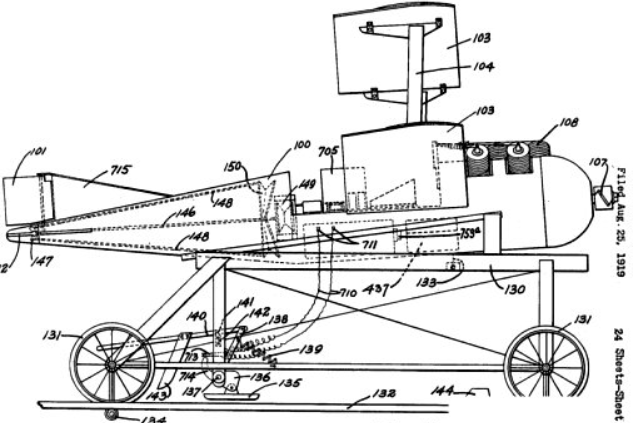
\includegraphics[scale=0.5]{imagenes/EstadodelArte/ketbug.png}
	\caption{Patente del Kettering Bug}
	\label{fig:Kettering Bug}
\end{figure}
 
Los drones que conocemos hoy en día eran llamados \textit{UAV} (Vehículos aéreos no tripulados). Los UAV con fines de reconocimiento se desplegaron por primera vez a gran escala en la Guerra de Vietnam. En esta época también comenzaron a usarse en una variedad de nuevos roles, como actuar de señuelos en combate, lanzar misiles contra objetivos fijos y lanzar folletos para operaciones psicológicas. 

Después de la Guerra de Vietnam, otros países fuera de Gran Bretaña y Estados Unidos comenzaron a explorar la tecnología de los \textit{UAV}. Los nuevos modelos se volvieron más sofisticados, con una resistencia mejorada y la capacidad de mantener una mayor altura. En los últimos años, se han desarrollado modelos que utilizan tecnología como la energía solar para abordar el problema de alimentar vuelos más largos. \newline

Los drones ahora tienen muchas funciones, que van desde monitorear el cambio climático hasta llevar a cabo operaciones de búsqueda después de desastres naturales, fotografía, filmación y entrega de bienes. Pero su uso más conocido y controvertido es el uso militar para reconocimiento, vigilancia y ataques dirigidos. Desde los atentados terroristas del 11 de septiembre, Estados Unidos aumentó significativamente el uso de drones, aplicándose posteriormente a un nivel global para la seguridad. Se utilizan principalmente para la vigilancia en áreas y terrenos donde las tropas no pueden ir con seguridad; aunque, tristemente también tienen un gran potencial ofensivo. \newline \cite{HistDrones} \cite{HistDrones2}


\subsection{Tipos}

Los drones están en su punto más alto y cada vez son más las empresas que definen sus productos como \textit{drones} , por lo que existe un gran abanico de posibilidades en cuanto a su clasificación. \cite{TipoDron} Sin embargo la más extendida son \textbf{según su uso} y \textbf{según el tipo de ala.} \newline

Según su uso: 

\begin{itemize}
	\item \textbf{Uso Militar.} Se usan con fines de reconocimiento, como ofensiva e incluso reabastecimiento de provisiones. En este campo se pueden incluir los usados por la policía.
	\item \textbf{Uso Comercial.} Se encuentran desde los usados como diversión hasta los usados para publicidad,etc.
\end{itemize}

Según el tipo de ala:

\begin{itemize}
	\item \textbf{Drones de ala fija \ref{fig:Alafija}.} Estos drones proporcionan una gran autonomía durante el vuelo ya que son muy aerodinámico; sin embargo necesitan mucho espacio para aterrizar y un sistema de lanzado para despegar, lo que los hace muy engorrosos. Se utilizan sobre todo para hacer mapas y labores de riego
\begin{figure}[H]
	\center
	\includegraphics[scale=0.125]{imagenes/EstadodelArte/Alafija.png}
	\caption{Ala fija}
	\label{fig:Alafija}
\end{figure}
 
	\item \textbf{Drones de ala rotatoria\ref{fig:Alarotatoria}.} Son los más extendidos en el ámbito comercial. A diferencia con los de ala fija estos pueden permanecer suspendidos en el aire gracias al sistema de hélices que llevan; no obstante tienen mucha menos autonomía que los de ala fija haciéndolos útiles solo para vuelos cortos. Cómo se pueden mantener estables gracias a sus giroscopios y estabilizadores son ideales para sacar fotos y hacer vídeos.
\begin{figure}[H]
	\center
	\includegraphics[scale=0.1]{imagenes/EstadodelArte/Alarotatoria.png}
	\caption{Ala rotatoria}
	\label{fig:Alarotatoria}
\end{figure}
 
\end{itemize}

Dentro de cada tipo, cada dron cuenta con un receptor radio determinado. A la hora de elegir el dron para nuestro proyecto será importante mirar las especificaciones del receptor radio que posee, ya que las comunicaciones entre el dron y la emisora (En este caso la FPGA) puede funcionar con distintos protocolos de comunicaciones. 

\subsection{Protocolos de comunicaciones de un dron}\label{sec:comdron}

En el ámbito de los drones, las más importantes son PWM, PPM y PCM.

\subsubsection{Modulación por ancho de pulsos (PWM)}

La modulación por ancho de pulsos o PWM es un método que permite generar una señal analógica desde un sistema digital.  Una señal de PWM es periódica y tiene dos elementos principales: un ciclo de trabajo y una frecuencia. \newline El ciclo de trabajo describe la cantidad de tiempo que la señal está en estado alto, como un porcentaje con respecto a la cantidad de tiempo que está en estado bajo. La frecuencia determina cómo de rápido la señal completa un ciclo, y por lo tanto que tan rápido cambia entre los estados alto y bajo.  Este ciclo de trabajo será modificado para transmitir una información o controlar la energía de la señal enviada, mientras que la frecuencia debe ser siempre la misma para poder medir el tiempo que la señal está en alto. 

\begin{figure}[H]
	\center
	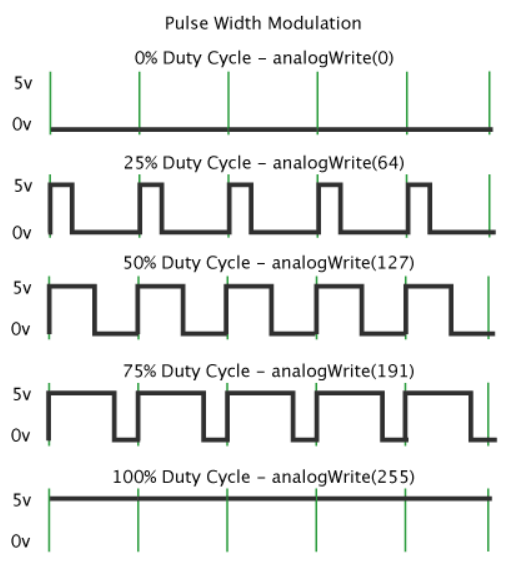
\includegraphics[scale=0.7]{imagenes/EstadodelArte/pwm.png}
	\caption{Modulación PWM}
	\label{fig:PWM}
\end{figure}

Esta modulación se utiliza mucho en la industria(ya que es la más común y generalmente la más barata.), y es con la que se controlan la mayoría de los servos en la robótica. 
Cada canal tiene su propio cable único, por lo que si tiene un receptor de 8 canales necesitará conectar 8 cables para leer las entradas en su controlador de vuelo.

\subsubsection{Modulación de posicion de puntos (PPM)}
En la Modulación por Posición de Pulso o PPM la amplitud y el ancho son fijos, pero la posición del pulso es variable. Es un tipo de modulación en la cual una palabra de M bits se codifica para la transmisión de un pulso que se encuentra en las N posiciones posibles,  donde N corresponde al tipo de modulación PPM (N-PPM).
\begin{equation} 
N=2^M 
\end{equation} 
La ventaja de PPM es que solo se necesita un cable de señal para varios canales (típicamente 8 canales como máximo), en lugar de varios cables individuales. Por lo tanto, solo debe conectar el cable de tierra, alimentación y señal.

\begin{figure}[H]
	\center
	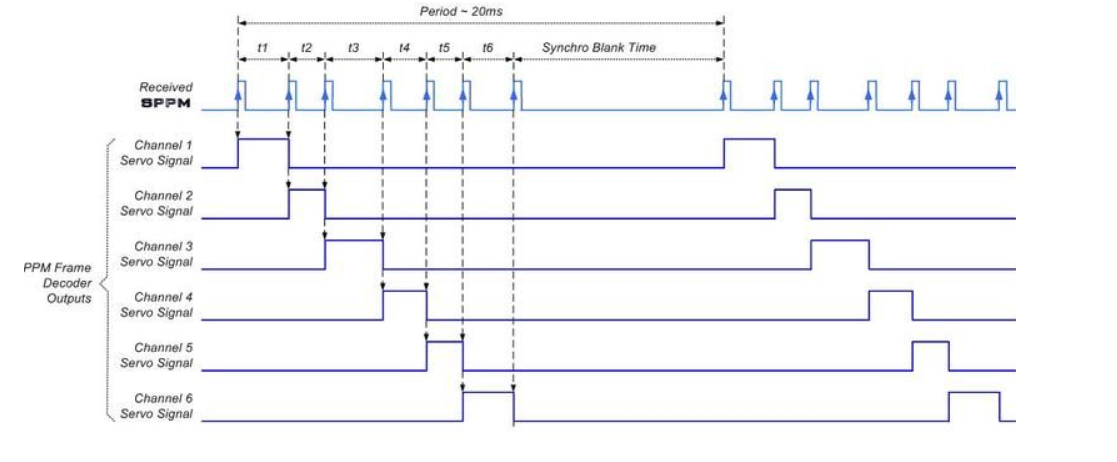
\includegraphics[scale=0.5]{imagenes/EstadodelArte/ppm.png}
	\caption{Modulación PPM}
	\label{fig:PWM}
\end{figure}

\subsubsection{Modulación de código de pulso (PCM)}

La modulación de código de pulso o PCM, es un tipo de modulación similar a PPM; sin embargo, la señal modulada en PCM es una señal digital (usando unos y ceros) mientras que la señal PPM es analógica. La modulación PCM tiene un gran potencial de detección de errores e incluso de corrección, es más confiable y menos susceptible a las interferencias; no obstante, requiere varias conversiones adicionales para su funcionamiento lo que se traduce en equipos muy costosos.


\section{Bioseñales y el EMG}

Entendemos por bioseñal \cite{nait2009advanced} cualquier señal de los seres vivos que se puede medir así como monitorear. Normalmente el término bioseñal se usa para refirse a señales bioeléctricas variantes en el tiempo; pero puede usarse también para señales no eléctricas, como por ejemplo la termografía o la respiración.\newline

Estas bioseñales eléctricas generalmente se caracterizan por un cambio de corriente eléctrica; producido por la diferencia de potencial eléctrico a través de un tejido, órgano o sistema. Entre las más conocidas tenemos: 

\subsubsection{Electrocardiograma}

Un \textit{electrocardiograma} \cite{subramanian2017ecg} (ECG) es el registro de la actividad eléctrica del corazón durante un período de tiempo, utilizado por los médicos para predecir y tratar diversas enfermedades cardiovasculares. Se capta a través de unos electrodos en la piel que detectan la despolarización y repolarización del corazón durante cada latido cardíaco, lo que proporciona una visión de la actividad muscular del corazón. \newline

Un trazado de ECG típico es un ciclo de tres entidades:

\begin{itemize}
	\item \textbf{La onda P}, que representa la despolarización de las aurículas.
	\item \textbf{El complejo QRS}, que representa la despolarización de los ventrículos .
 	\item \textbf{La onda T}, que representa la repolarización de los ventrículos.
\end{itemize}

\begin{figure}[H]
	\center
	
\includegraphics[scale=0.1]{imagenes/EstadodelArte/ECG.png}
	\caption{ECG de un corazón en ritmo sinusal normal}
	\label{fig:ECG}
\end{figure}
 

\subsubsection{Electroencefalografía}

La \textit{electroencefalografía} (EEG) mide la actividad eléctrica del cerebro, registrada a partir de electrodos colocados en el cuero cabelludo. Cuando se analizan estas señales, se utilizan como una herramienta de diagnóstico para detectar patologías asociadas con un comportamiento eléctrico extraño.  Se usa con mayor frecuencia para diagnosticar la epilepsia , lo que causa anormalidades ev en las lecturas del EEG. También se usa para diagnosticar trastornos del sueño , profundidad de la anestesia , coma , encefalopatías y muerte cerebral.

\begin{figure}[H]
	\center
	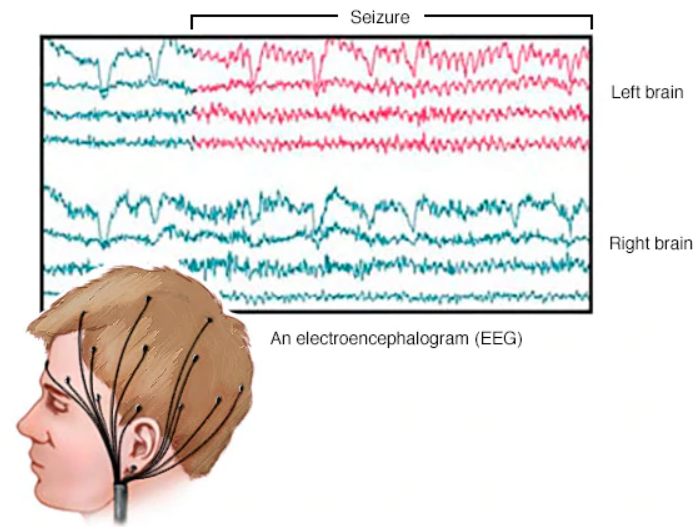
\includegraphics[scale=0.7]{imagenes/EstadodelArte/EEG.png}
	\caption{EEG y colocación de los electrodos}
	\label{fig:EEG}
\end{figure}
 

\subsubsection{Electromiograma}

La \textit{electromiografía} ( EMG ) es una técnica de medicina electrodiagnóstica para evaluar y registrar la actividad eléctrica producida por los músculos esqueléticos . Cada vez que se ejecutan los músculos del cuerpo para una determinada actividad, el cerebro envía señales de excitación a través del \textit{sistema nervioso central}. Los músculos están inervados en grupos llamados \textit{unidades motoras}, que son el punto de unión donde se encuentran la neurona motora y las fibras musculares.  Cuando la \textit{unidades motora} se activa, produce un potencial de acción y el sistema nervioso central se activa continuamente durante el tiempo que se requiera que el músculo genere fuerza. Este \textit{potencial de acción de la unidad motora} es la señal EMG que vemos resultante.

Para obtener el EMG se utiliza un electromiógrafo, el cuál detecta el potencial eléctrico generado por las células musculares cuando estas células se activan eléctrica o neurológicamente. En el ámbito médico por lo tanto el EMG se utiliza como herramienta de diagnóstico para enfermedades neuromusculares, pero sus usos se han ampliado actualmente a la rehabilitación de pacientes en forma de prótesis robótica. \newline

Y es que en nuestros días un mecanismo róbótico con varios grados de libertad puede imitar perfectamente el movimiento de una extremidad humana. 

\begin{figure}[H]
	\center
	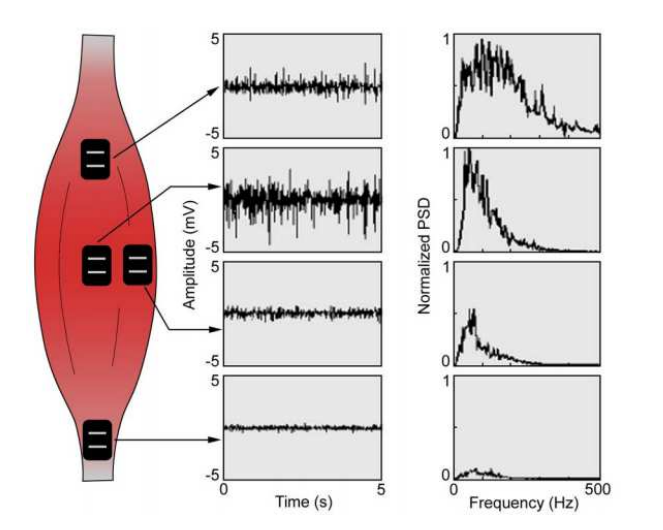
\includegraphics[scale=0.7]{imagenes/EstadodelArte/EMG.png}
	\caption{EMG y colocación de los electrodos}
	\label{fig:EMG}
\end{figure}

Se propone usar la bioseñal EMG en este proyecto debido a la facilidad para discriminar movimientos, que será lo que permita controlar el dron y definir su comportamiento. Sin embargo, antes de poder usar la señal EMG hay que tener varios factores en cuenta, que va desde su captación hasta las posibles interferencias que pueden acusar a este tipo de señal. \ref{sec:Ruido}

\subsection{Tipo de señal y ruido}\label{sec:Ruido}

Antes de pasar a la fase de adquisición de la señal, es importante familiarizarse con los distintos factores que afectan a las propiedades cualitativas de la señal.\newline

Una señal de EMG tiene las siguientes características:
\begin{itemize}
	\item La amplitud de la señal EMG se encuentra entre 1-10 mV, lo que la convierte en una señal considerablemente débil. 
	\item La señal se encuentra en el rango de frecuencia de 0-500 Hz y la más dominante es entre 50-150 Hz.
	\item La señal EMG está muy influenciada por el \textit{ruido:}\newline
	\begin{itemize}
		\item El ruido ambiental puede ser causado por fuentes de radiación electromagnética, por ejemplo, dispositivos de transmisión de radio, luces fluorescentes y la interferencia de la línea de alimentación de los cables eléctricos. Estas interferencias son casi imposibles de evitar por medios externos. Este ruido particular 			existe en el rango de frecuencia de 50-60 Hz. \newline
		\item El ruido también se puede generar a partir de artefactos de movimiento. Las dos fuentes principales de este ruido son la inestabilidad de la interfaz de la capa del electrodo y el movimiento del cable del electrodo y se encuentra principalmente en el rango de 0-20 Hz. Se puede eliminar mediante un conjunto 					adecuado de equipos y circuitos de EMG. La máxima fidelidad de la señal está determinada por la relación señal / ruido EMG adquirida. \newline
	\end{itemize}
\end{itemize}

El kit biosignalplux nos va a permitir adquirir las señales EMG y poder ver la interacción eléctrica en tiempo real. Este kit será el que utilicemos para obtener las señales EMG y procesarlas posteriormente.





\chapter{Herramientas software y hardware}\label{sec:Herramienta_software _y _hardware}
\section{Biosignalplux}
Para la adquisición usaremos el kit de investigación de Biosignalplux de 8 canales. Utiliza el software OpenSignals para adquirir y visualizar simultáneamente hasta 8 sensores de EMG. \newline
\begin{figure}[H]
	\center
	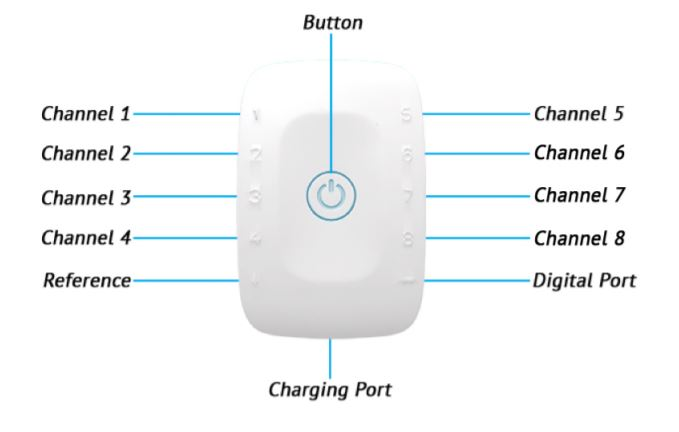
\includegraphics[scale=0.8]{imagenes/Herramientas/Bios.jpg}
	\caption{Hub de Biosignalplux}
	\label{fig:Biosignalplux}
\end{figure}
 
\section{Matlab}
Es un programa de cálculo numérico el cual cuenta con su propio lenguaje de programación. Permite la comunicación con dispositivos hardware así como la visualización y programación de manera fácil e intuitiva dónde las soluciones se expresan como funciones matemáticas. Como ventaja permite resolver problemas computacionales en un tiempo menor de lo que tardaría un lenguaje escalar no interactivo como C. \newline
\section{FPGAS}
Una FPGA (Field Programmable Gate Array) es un dispositivo programable con bloques lógicos cuya interconexión puede ser configurada mediante un lenguaje de descripción para crear circuitos digitales.\newline

Están compuestos internamente por puertas lógicas, cables y biestables; todo ello sin conectar, como una plantilla en blanco. Para su programación requiere la carga de un archivo con la descripción del circuito - o bitstream- que define las uniones entre los biestables y puertas lógicas para crear el circuito que deseemos. 

\begin{figure}[H]
	\center
	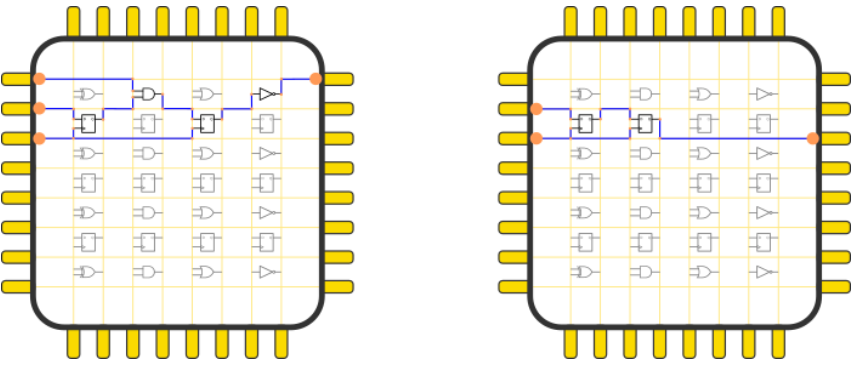
\includegraphics[scale=0.6]{imagenes/Herramientas/FPGA.png}
	\caption{Estructura interna de una FPGA}
	\label{fig:Estructura interna de una FPGA}
\end{figure}

\subsection{FPGAs vs MCU}

Las FPGA y los MCU (microcontroller unit - microcontrolador) son dos de las herramientas más poderosas disponibles para un ingeniero eléctronico en la actualidad. Es esencial para cualquier persona que trabaje en electrónica digital, como para un profesional en cualquier industria, o incluso un aficionado, obtener una comprensión completa de las herramientas disponibles para ayudar en su trabajo. Esto es especialmente cierto en una industria acelerada, donde las herramientas y tecnologías están sujetas a cambios repentinos y frecuentes.\newline

\begin{figure}[H]
	\center
	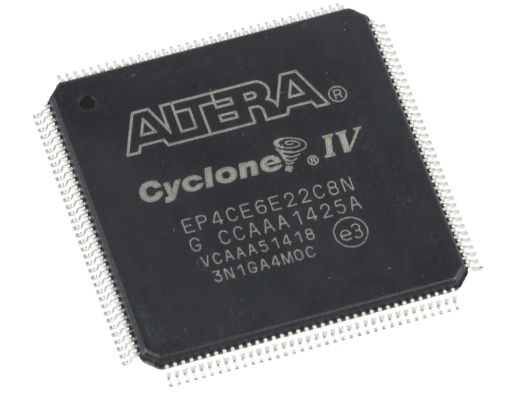
\includegraphics[scale=0.6]{imagenes/Herramientas/FPGA2.png}
	\caption{FPGA EP4CE6E22C8N}
	\label{fig:FPGA EP4CE6E22C8N}
\end{figure}


\begin{figure}[H]
	\center
	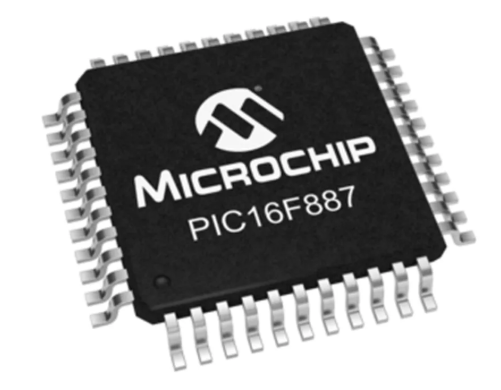
\includegraphics[scale=0.6]{imagenes/Herramientas/MCU.png}
	\caption{MCU PIC16F887}
	\label{fig:MCU PIC16F887}
\end{figure}


Estos dispositivos se usan generalmente en escenarios muy similares; para decirlo de manera muy amplia: los dos permiten introducir unos valores de entrada y obtener los cambios que deseemos en las salidas. De hecho, casi cualquier aplicación que use un microcontrolador podría emplearse en una FPGA para el mismo efecto, y viceversa. Esto no quiere decir que las dos tecnologías sean intercambiables; a veces lo que es muy difícil lograr usar en un dispositivo, podría ser una cuestión simple para el otro.\newline 

La diferencia más importante entre los microcontroladores y las FPGAs es la forma en que procesan las instrucciones. Los primeros  procesan comandos secuencialmente, lo que significa que un micro lee cada línea del programa de una en una, en secuencia. Por el contrario, los FPGA procesan comandos simultáneamente, por lo que las líneas de código se ejecutan a la vez; traduciéndose en un incremento de la velocidad. Además en un microprocesador cada instrucción está asociada a un hardware de manera fija, y el programador no puede usar más instrucciones de las que le ofrece el fabricante. Las FPGAs no tienen nada conectado de manera fija, el usuario es el que determina mediante conexiones el comportamiento del circuito. \newline
Debido a esto las FPGAs generalmente se usan en escenarios que requieren un procesamiento de datos en paralelo de alta velocidad, o un alto grado de personalización, pero pueden resultar engorrosas por su relativa complejidad de configuración. Mientras tanto, los MCU son mucho más fáciles de configurar y usar desde el principio, manejan de manera aceptable los datos en serie de alta velocidad y su producción es más barata. \newline

Sin embargo, el panorama actual de los MCUs está a punto de cambiar debido al estancamiento de la ley de Moore. \newline

\subsubsection{El estancamiento de la ley de Moore}

La Ley de Moore es la observación empírica realizada el 19 de abril de 1965 por Gordon Moore, cofundador de Intel , en la que postulaba que el número de transistores por unidad de superficie de un microprocesador iba a duplicarse cada 2 años- y por lo tanto la velocidad del procesador o la potencia de procesamiento general-, al menos durante las siguientes dos décadas.\newline

\begin{figure}[H]
	\center
	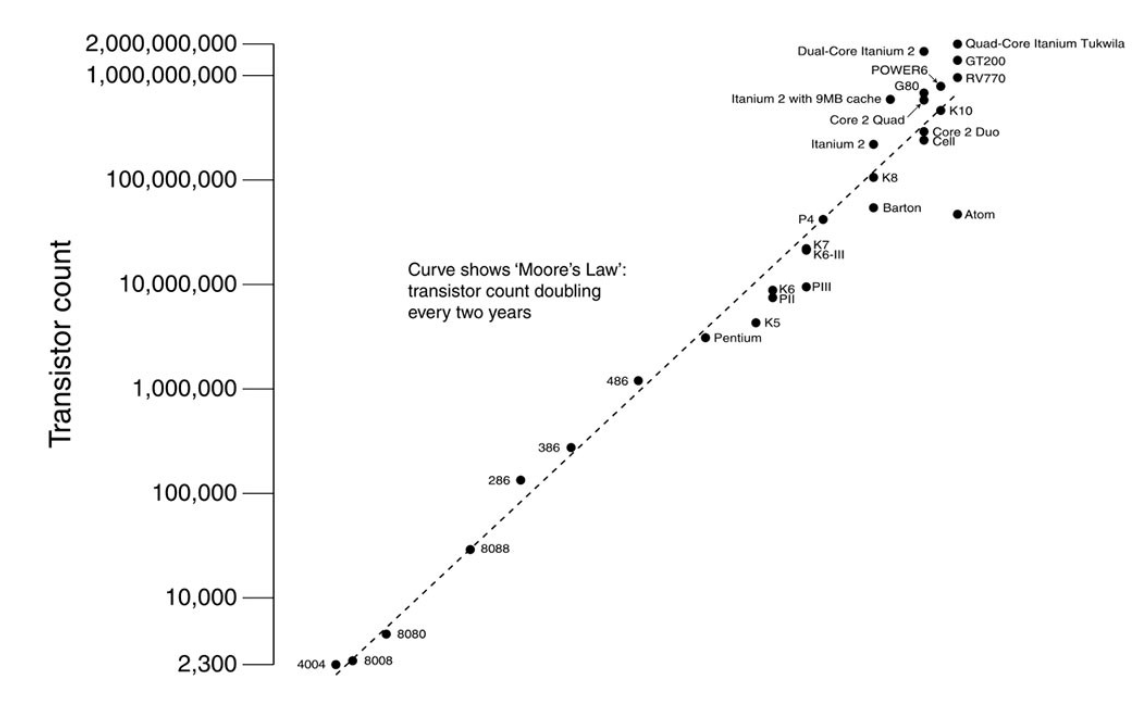
\includegraphics[scale=0.6]{imagenes/Herramientas/leymoore.png}
	\caption{La ley de Moore}
	\label{fig:La ley de Moore}
\end{figure}

La mayoría de los expertos, incluido el propio Moore esperan que esta apreciación se mantenga vigente hasta 2020-2025 donde dejará de cumplirse definitivamente . El estancamiento de la ley de Moore es la consecuencia de los límites físicos de la tecnología actual, en la que un número mayor de transistores para un mismo volumen se traduce en un mayor calor generado que no se va a poder disipar sin dañar el microcontrolador (Enfriar los transistores requiere más energía de la que pasa por los transistores).
 Este estancamiento de la tecnología de los microprocesadores, hará que no se pueda equiparar la potencia a la continua mejora de la velocidad de sus algoritmos; por lo que será necesario la búsqueda de nuevas tecnologías para que las empresas puedan seguir desarrollando sus productos.\newline

Aquí es donde entran en juego las FPGAs y el hecho de la importancia que están adquiriendo para las empresas su uso; ya que les permite multiplicar por un factor considerable la velocidad en sus circuitos. Las FPGAS se conocen desde los años 80, pero era una tecnología cerrada que muy pocos podían usarla; además, las herramientas para manejarlas eran complejas de usar. Todo cambió con la llegada de las FPGAS "libres", que ha propiciado que muchos aficionados creen herramientas para poder usarlas de una manera más intuitiva y sencilla. \newline

\subsection{FPGAS libres}

El término “libre” se refiere a los productos que se han diseñado específicamente para que sean totalmente accesibles para todos los usuarios, disponiendo de total libertad para utilizar, modificar y trabajar con estos productos. 
Las ventajas que permiten son enormes para el patrimonio tecnológico. Normalmente son mucho más fiables ya que hay un gran número de usuarios que trabajan para hacer que llegue a más gente. \newline

A las FPGAs les llegó su momento en mayo del 2015, en el panorama cambió con el Proyecto IceStorm creado por el ingeniero austríaco Clifford Wolf. Wolf hizo ingeniería inversa de una de la FPGA ICE40 de Lattice para obtener toda la información de funcionamiento y poder crear herramientas libres que no dependieran de ningún fabricante. Esto permitió un gran desarrollo del sector ya que rápidamente se creó una gran comunidad.
La placa que usaremos para el proyecto será la Icezum Alhambra, pero existe una amplia variedad de placas con FPGAs libres.

\subsubsection{Icezum Alhambra II}

Tras un pequeño estudio del mercado de las FPGAs libres, la placa Icezum Alhambra II será la que utilicemos para este proyecto. Tanto la primera versión como la revisión fueron diseñadas en Pinos del Valle(Granada) por Eladio Delgado. Sus dimensiones y apariencia es muy similar al de la placa Arduino UNO; ya que el objetivo era que fuera compatible con la mayoría de Shields de Arduino, que son placas de circuitos modulares que le dan funcionalidades extras. Además, al igual que Arduino es una placa que está pensada para el aprendizaje y la docencia, por lo que cuenta con bastantes añadidos como LEDs y pulsadores para que sea más fácil y cómodo su uso para pequeños proyectos.

\begin{figure}[H]
	\center
	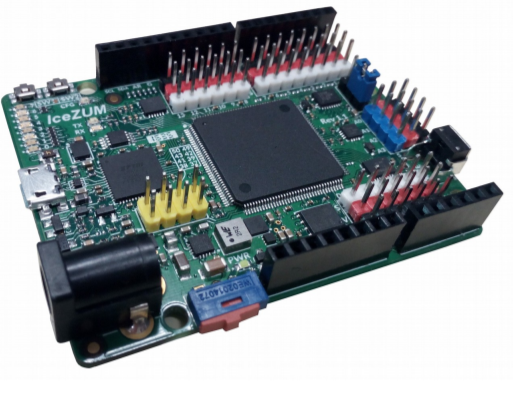
\includegraphics[scale=0.6]{imagenes/Herramientas/Icezum.png}
	\caption{Icezum Alhambra II}
	\label{fig:Icezum Alhambra II}
\end{figure}

Las características principales de la Icezum Alhambra II son:

\begin{itemize}

	\item Placa de desarrollo con FPGA iCE40HX4K (Lattice) 
	\item Hardware abierto
	\item Compatible con Icestudio
	\item Se pueden reutilizar la mayoría de los shield disponibles en Arduino
	\item Placa recomendada para proyectos robóticos
	\item El dispositivo USB FTDI 2232H permite la programación de la FPGA y la interfaz UART la conexión a un PC
	\item Interruptor electrónico de encendido/apagado
	\item 8 LED de uso general (LED de usuario)
	\item 2 botones de propósito general
	\item Memoria flash de 32 Mb 
	\item 20 pines de entrada / salida de 3.3V (tolera 5V)
	\item Todos los pines de E/S incluyen resistencias en serie de 200 ohmios para la activación directa de LED
	\item Convertidor A/D de 4 canales y 12 bits
	\item Pines de arranque en frío accesibles desde GPIO
	\item Reguladores de conmutación para procesamiento de alta frecuencia a baja potencia de entrada
	\item Oscilador MEMS de 12 MHZ
	\item Botón de reinicio
	\item Fuente de alimentación USB, dos conectores (hasta 4.8A)
\end{itemize}


\begin{figure}[H]
	\center
	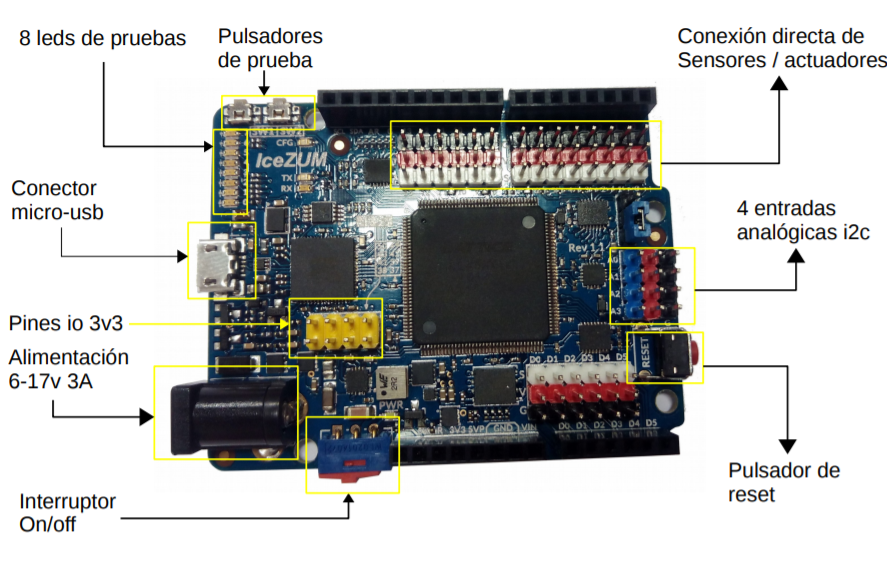
\includegraphics[scale=0.6]{imagenes/Herramientas/Icezum2.png}
	\caption{Icezum Alhambra II}
	\label{fig:Icezum Alhambra II}
\end{figure}


\subsubsection{Icestudio}

Icestudio se trata de un editor visual para FPGAs libres, el cual permite el diseño de forma bastante sencilla para FPGAs mediante la creación de bloques con funcionalidades definidas. Icestudio utiliza el lenguaje de descripción hardware Verilog para la creación de estos bloques, que se muestra al usuario como puertas lógicas y biestables.  La interfaz es la siguiente:


 \chapter{Diseño del sistema} 

Para realizar el procesamiento más adecuado al sistema, en primer lugar se tendrá que entrenar con una serie de señales obtenidas de \textit{prueba} con tal fin. Una vez captadas y ajustado el algoritmo, probaremos con una batería de señales en cada brazo que este funciona como lo esperado y cumple con su objetivo. Con estos datos ya no se modificará el algoritmo de procesamiento. 

\begin{figure}[H]
	\center
	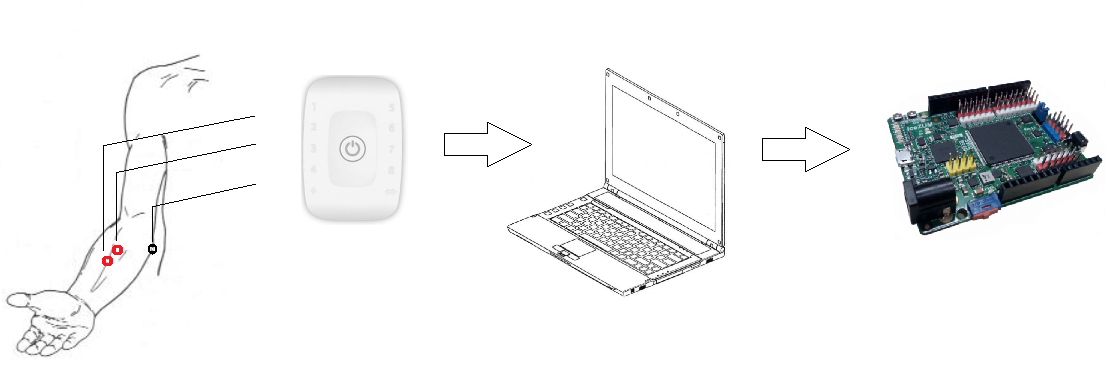
\includegraphics[scale=0.6]{imagenes/Disenodelsistema/sistema.png}
	\caption{Proceso para obtener y procesar bioseñales}
	\label{fig:Sistema}
\end{figure}


En primer lugar se captan las señales de prueba o entrenamiento, que mediante Bluethooth son enviadas al ordenador en tiempo real y recogidas en el software OpenSignals. Estas señales que hemos guardado son posteriormente procesadas en Matlab para su filtrado y captación de parámetros que nos permitan distinguir los distintos estados en los que se encuentra el músculo. El filtrado debe de ser capaz de eliminar el ruido y de acondicionar la señal para que sea más fácil distinguir sus parámetros de bondad. 
 \newline
Una vez las señales se procesan son enviadas mediante comunicación serie a la FPGA, en la que se va a definir el modo de control. Para ello se utilizará la modulación PWM, que como hemos visto en \ref{sec:comdron} es la tecnología más barata y utilizada. 

En los siguientes capítulos vamos a ver más detenidamente todo el proceso de obtención así como la implementación del proyecto.

\section{Adquisición}

En cuanto a la adquisición de señales EMG hay que tener en cuenta un correcto acondicionamiento de la piel y una colocación adecuada de los electrodos de medida.

\subsection{Preparación de la piel} \label{sec:Preparaciondelapiel}
 Es necesario a la hora de obtener señales EMG una correcta preparación de la piel dónde vamos a colocar los electrodos; de forma que la calidad de la señal obtenida sea la mejor posible. Para este propósito es recomendable usar un gel abrasivo o alcohol tanto para eliminar las células muertas de la piel como para reducir la sequedad de la misma. Tras la correcta limpieza con un paño suave se asegura que la zona quede totalmente limpia y seca. \newline
\subsection{Los electrodos} \label{sec:Loselectrodos}
Para ello se usan 3 electrodos  (2 y uno de referencia) que se colocan directamente sobre la piel y son capaces de captar la actividad bioeléctrica. La ubicación de los electrodos va a influir directamente sobre la calidad de las señales obtenidas; una correcta colocación sería en paralelo a las fibras musculares, en la zona central del músculo del que queramos obtener la actividad eléctrica. Estos deberán estar separados de 1 a 2 cm y el de referencia deberá estar colocado en un sitio dónde sepamos que la actividad será minima; en los tendones y el borde del músculo las fibras musculares se vuelven más delgadas y pequeñas por lo que son el sitio ideal para colocar el electrodo de referencia. 

Antes de colocar los electrodos se puede usar una pasta conductiva que mejora considerablemente la captación de estos de las señales.\newline

\begin{figure}[H]
	\center
	\includegraphics[scale=0.8]{imagenes/Disenodelsistema/electrodo.png}
	\caption{Posición de los electrodos}
	\label{fig:Posicion}
\end{figure}

\subsection{Obtención de señales}

Con lo visto en \ref{sec:Preparaciondelapiel} y \ref{sec:Loselectrodos} tendríamos que definir el músculo que va a hacer de instrumento de control para el sistema. Se plantea la idea de usar un músculo del antebrazo por la facilidad para la colocación de los electrodos, así como a la hora de descriminar los distintos movimientos que nos van a permitir el control del sistema. Un correcto sitio sería con los 2 electrodos en la parte central y el de referencia en el codo que es un punto con poca actividad eléctrica.\newline 

El \textit{músculo flexor del carpo} (figura \ref{fig:flexor}) será  el que eligiremos debido a su posición central, ya que permite contraerlo y relajarlo con facilidad. \newline Por lo tanto este será el músculo sobre el cual vamos a colocar los electrodos para realizar la toma de señales y empezar a discriminar los distintos movimientos. Las pruebas deberán hacerse para los dos brazos, ya que nos permitirá más grados de libertad a la hora de elegir el método de control del sistema.  

\begin{figure}[H]
	\center
	\includegraphics[scale=0.5]{imagenes/Disenodelsistema/flexor.png}
	\caption{Músculo flexor del carpo en el antebrazo}
	\label{fig:flexor}
\end{figure}


Se tomarán unas señales EMG de entrenamiento, que mediante Bluethooth son enviadas al ordenador en tiempo real y vistas en OpenSignals. En el mismo OpenSignals podemos seleccionar el intervalo de tiempo de la captación que queremos guardar, y nos ofrece distintos formatos para hacerlo: .edf .h5 y .txt. Entre ellos guardaremos las señales como un archivo de texto (.txt), que tendrán el número de muestra y su valor correspondiente.\newline 

Estos archivos .txt será lo que lea Matlab para realizar el procesamiento. \newline


\begin{figure}[H]
	\center
	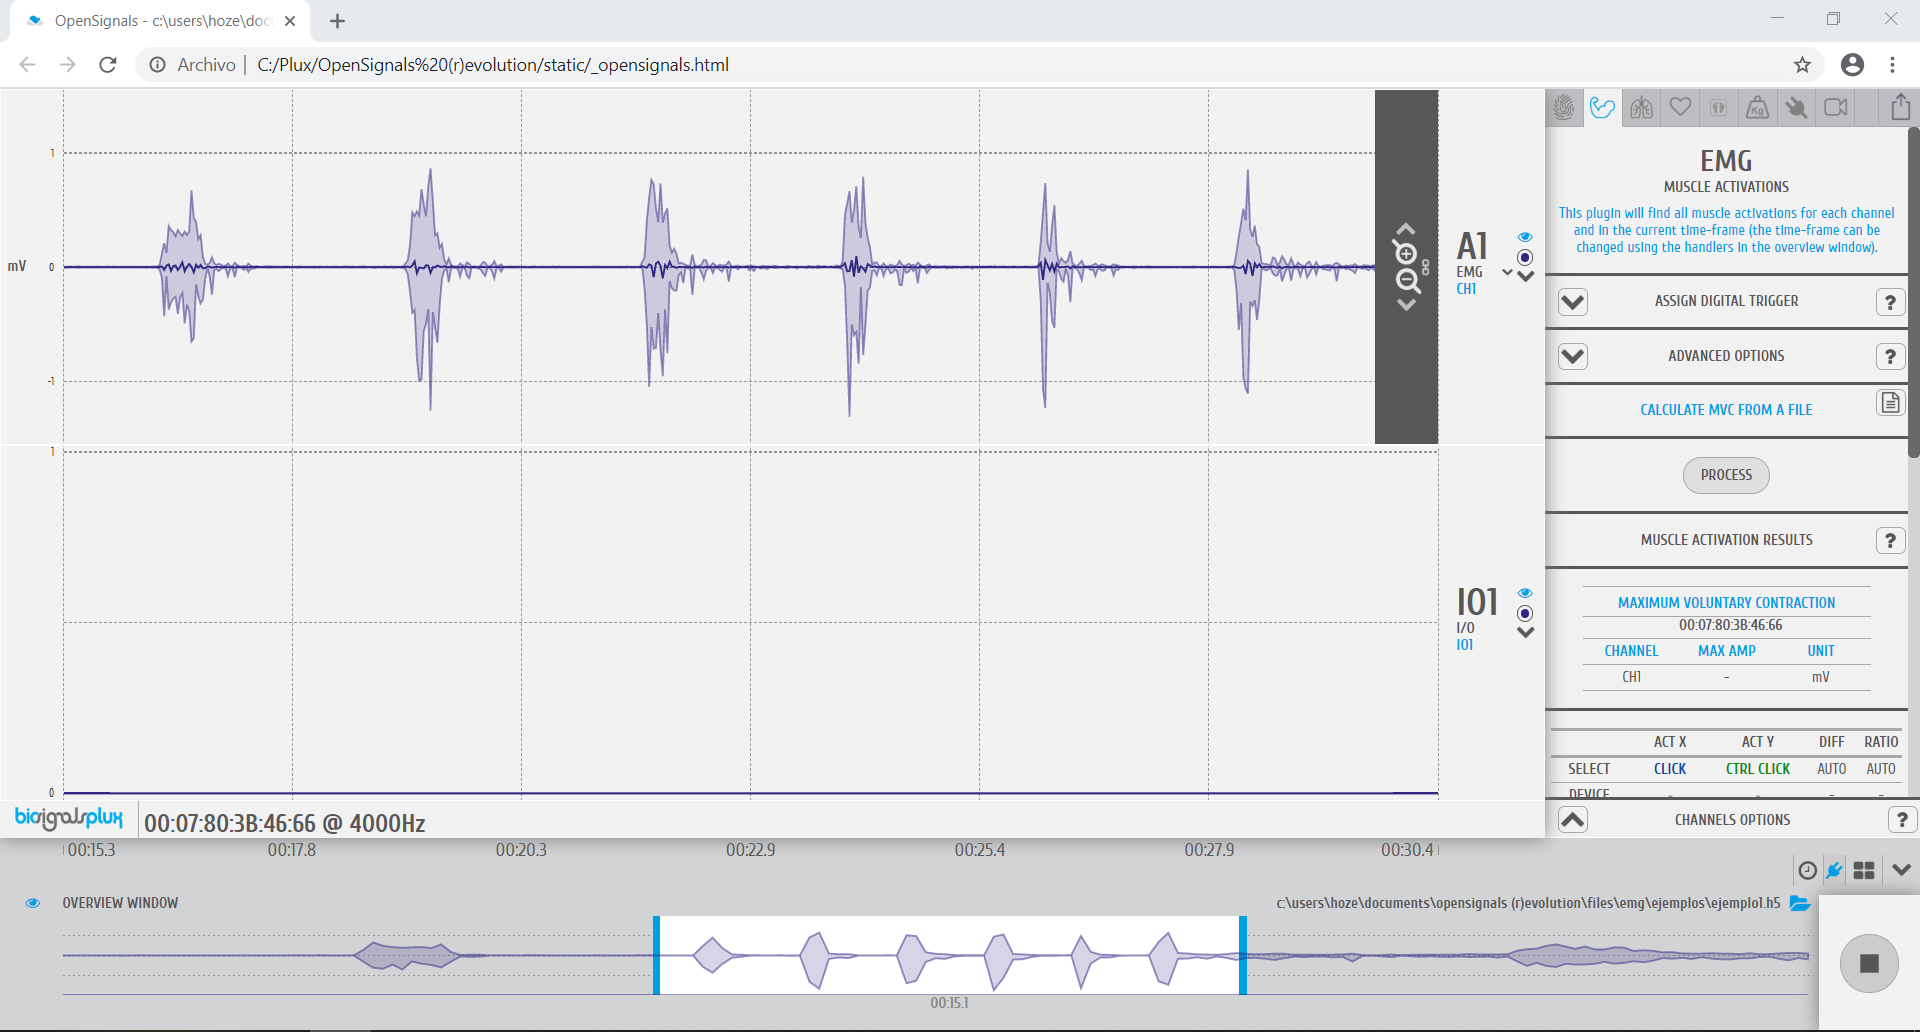
\includegraphics[scale=0.3]{imagenes/Disenodelsistema/ejemplo.png}
	\caption{Señal captada por OpenSignals}
	\label{fig:ejemplo}
\end{figure}



En la figura \ref{fig:ejemplo} se puede distinguir bastante bien las diferentes contracciones que ha sufrido el músculo en el proceso de obtención. Las zonas con una menor amplitud se tratan de relajaciones o momentos en los que el flexor se encuentra relajado y con poca actividad eléctrica. En el momento en el que contraemos voluntariamente el músculo se alcanzan picos de gran amplitud; que dependiendo de la fuerza de la contracción serán de mayor o menor intensidad. El algoritmo que creemos tendrá que ser carpaz por lo tanto de discriminar si el músculo se encuentra relajado o contraído.
Tras la obtención, un procesamiento con Matlab será necesario para acondicionarlas y preparar las señales para su uso.


\subsection{Procesamiento en Matlab}

A la hora de trabajar con bioseñales para el control de mecanismos robóticos, se necesitan señales sin interferencias. Las interferencias más comunes,como hemos visto en \ref{sec:Ruido} es el ruido de 50Hz de la red eléctrica; aunque también existen de otro tipo como las que ocurren en la medición, como el movimiento de los cables o incluso los problemas del mismo equipo que hace las medidas. \newline 

Para realizar el procesamiento digital de la señal EMG además será necesario tener en cuenta que la mayor parte de su información se encuentra en el rango de frencuencias de 5Hz a 500Hz. Debido a su comportamiento no determinista, debe procesarse con técnicas de caracterización que permitan conocer características definidas de la señal, a través de las cuales apicar los determinados métodos de control. \newline

Las señales en formato .txt son cargadas en Matlab mediante la función \textit{dlmread}, que lee los datos del fichero y los guarda en una matriz, donde el valor de la frecuencia de muestreo de la señal se almacena en una variable. Hay que tener en cuenta que los valores del fichero no son los valores reales de la señal, son valores muestreados que devuelve el programa; por lo que deben ser convertidos a voltaje usando una expresión matemática que nos facilita el manual de BioSignalplux.\newline

 La expresión matemática se define en \ref{eqn:ec1}:
\begin{equation}
EMG(V)=\frac{((ADC/2^n)-1/2)*Vcc}{G}
\label{eqn:ec1}
\end{equation}

Donde: 
\begin{itemize}
	\item Vcc= 3V (Voltaje de operación)
	\item G= 1000 (Ganancia del sensor)
	\item EMG(V) - Valor de la señal EMG en voltios
	\item ADC - Valor sampleado del canal que devuelve el programa
	\item n -Número de bits del canal
\end{itemize}


\begin{figure}[H]
	\center
	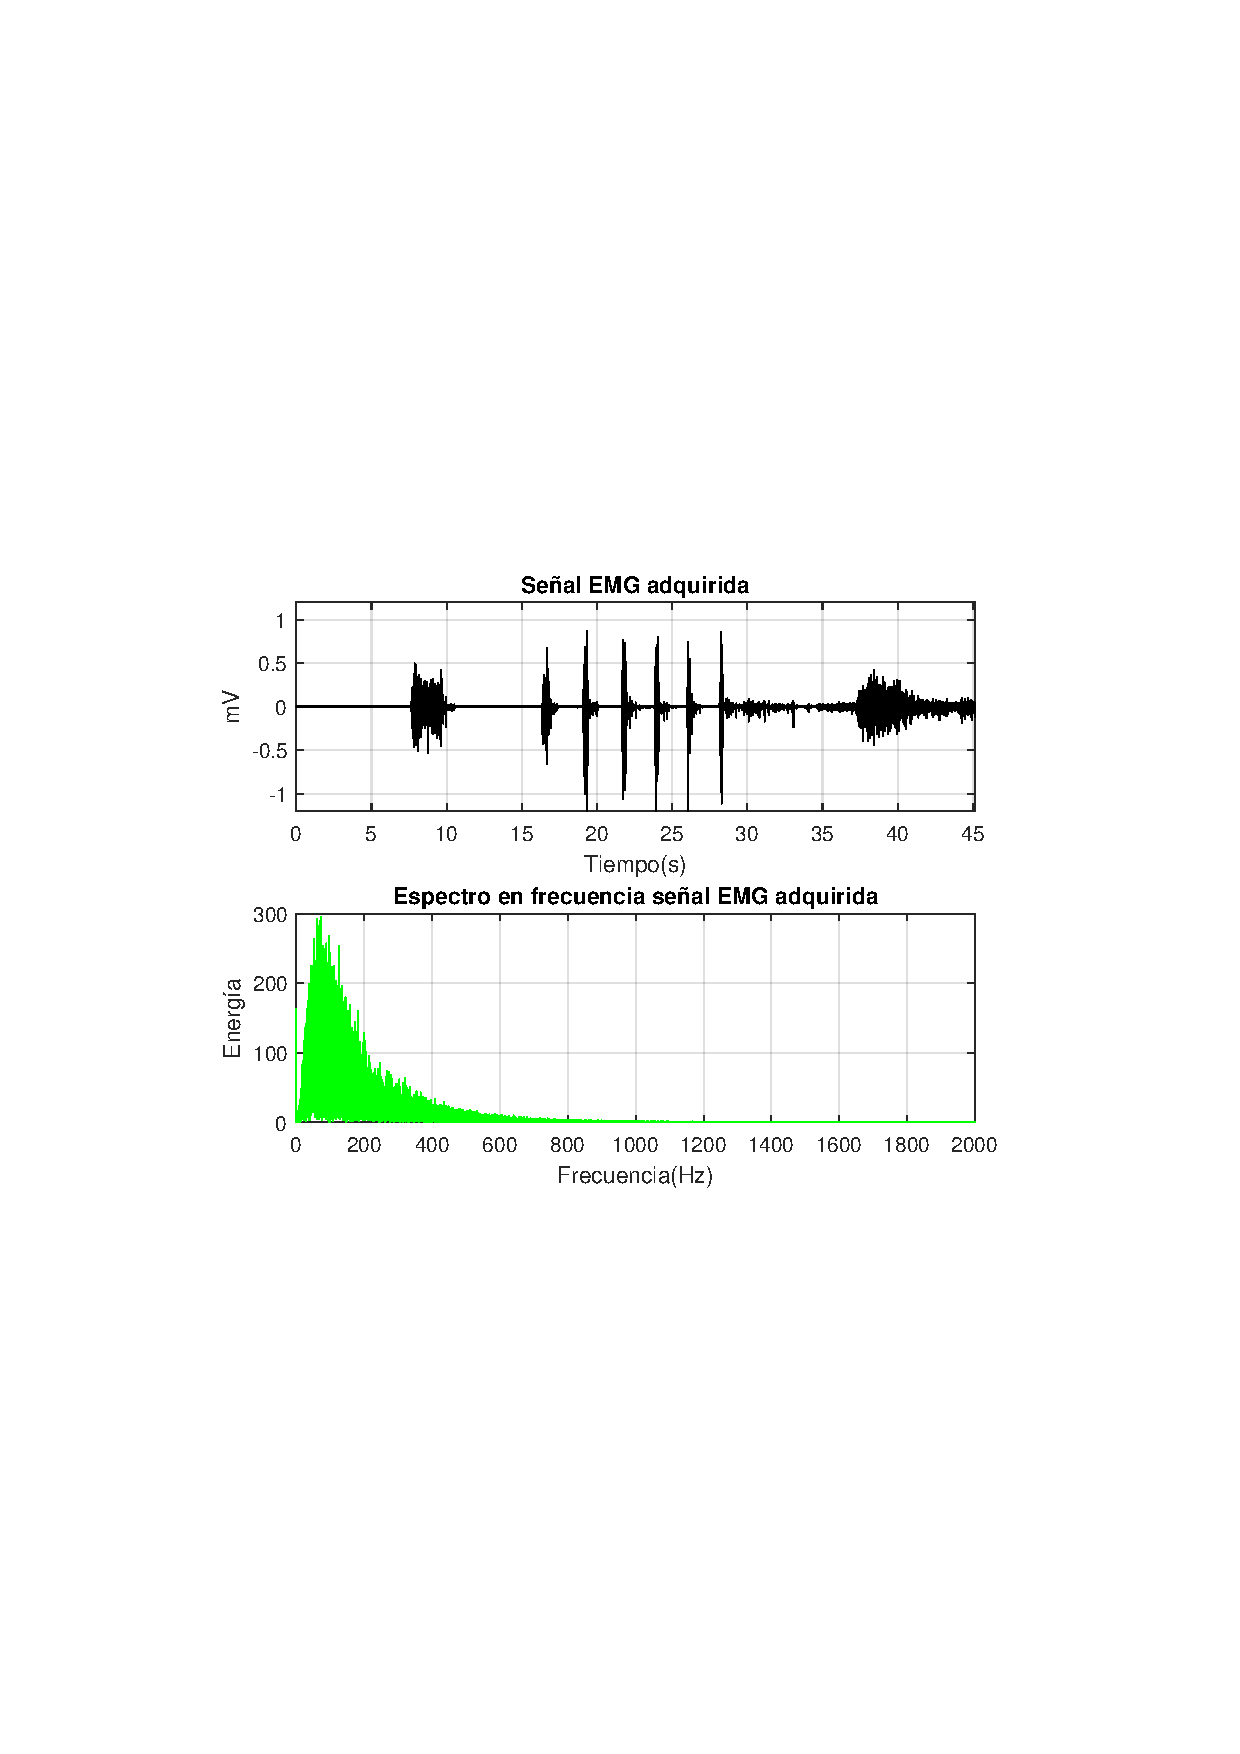
\includegraphics[scale=0.5]{imagenes/Disenodelsistema/graf1.png}
	\caption{Señal captada representada en Matlab}
	\label{fig:graf1}
\end{figure}

En la figura \ref{fig:graf1} se muestra la señal guardada una vez representada en Matlab en el dominio del tiempo y en el dominio de la frecuencia. Una vez tenemos la señal, si le hacemos la transformada rápida de fourier con el comando \textit{fft} podemos obtener su espectro correspondiente. Para que la señal sea óptima en las siguientes etapas será necesario filtrarla adecuadamente.

\subsubsection{Filtro de paso de banda EMG: 4Hz a 500Hz} \label{sec:pasobanda}

Como se ha comentado las señales EMG tiene su información más relevante en la banda de frecuencia entre 4Hz y 500Hz. Por esa razón, esto se toma como  criterio para el diseño de un filtro de paso banda, que puede ser entendido como un filtro pasa alto con frecuencia de corte de 4Hz en serie con un filtro paso bajo con frecuencias de corte de 500 Hz. \newline
Se elige que este filtro sea de Butterworth, ya que permite la respuesta más plana posible. Su función de transferencia es la siguiente:

\begin{equation}
|H(w)|^2 = \frac{1}{1+(w/wc)^(2N)}
\end{equation}

Donde: 
\begin{itemize}
	\item N es el orden del filtro
	\item wc es la frecuencia de corte 
	\item w la frecuencia compleja 
\end{itemize}

El filtro  de manera matemática puede ser complejo de calcular, pero Matlab cuenta con la función \textit{butter}  que lo hace automáticamente; especificando las frecuencias de corte y el orden del filtro. 
\begin{figure}[H]
	\center
	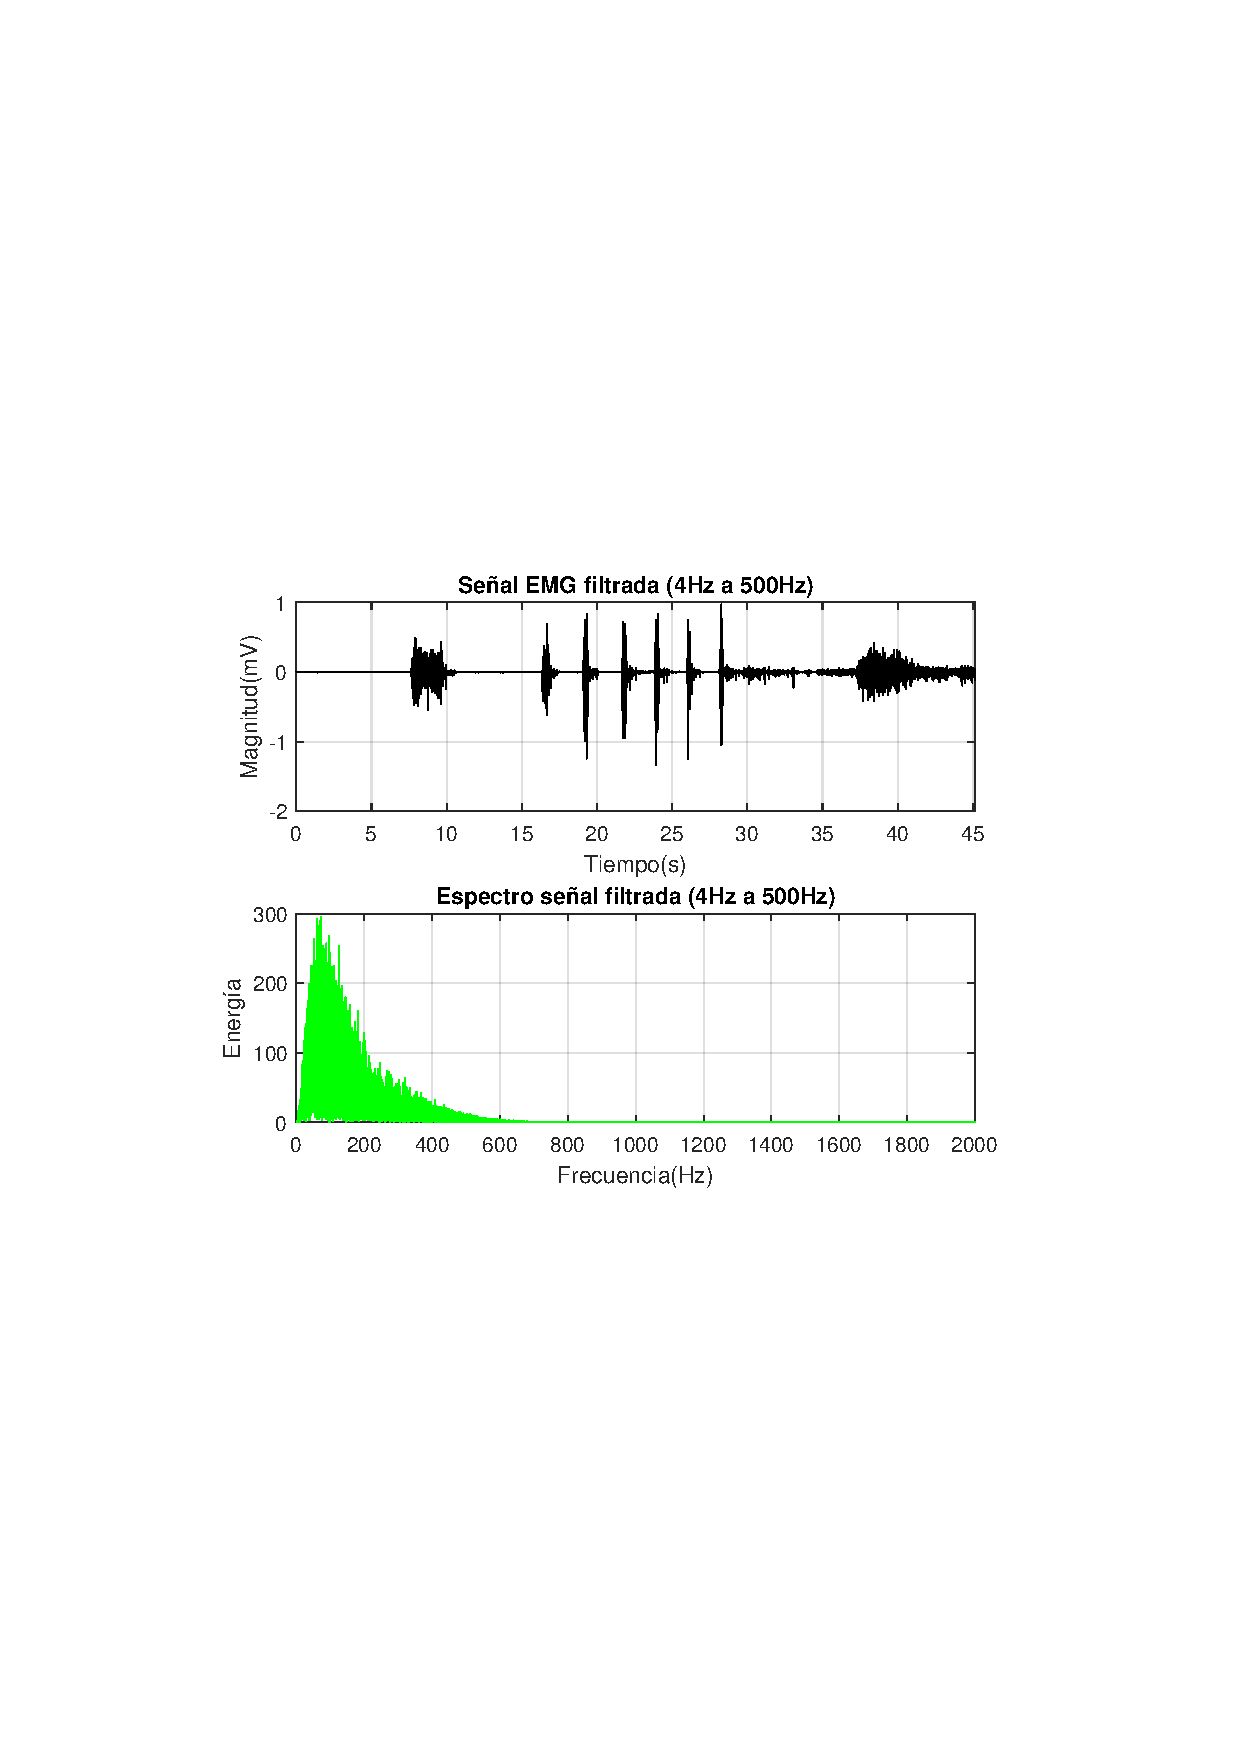
\includegraphics[scale=0.5]{imagenes/Disenodelsistema/graf2.png}
	\caption{Señal con el filtro paso banda}
	\label{fig:graf2}
\end{figure}

En la figura \ref{fig:graf2} la señal ya quedaría con la información más relevante en la banda 4Hz-500Hz, desechando las altas frecuencias que interfieran en la señal. 

\subsubsection{Filtro de rechazo banda EMG: 50Hz}

En España, la frecuencia de la línea eléctrica es de 50Hz, por lo que se requiere el diseño de un filtro rechazo banda que elimine este ruido. Se lleva a cabo el mismo procedimiento que en \ref{sec:pasobanda} para el diseño de un filtro de rechazo banda de 50Hz. Para ello se usa de nuevo la función \textit{butter} pero esta vez con el parámetro \textit{stop} para que sea de rechazo. Esta nueva filtración se añade a la anterior, dejando las señales libres de ruido y acondicionadas para sacar sus parámetros de bondad.

\begin{figure}[H]
	\center
	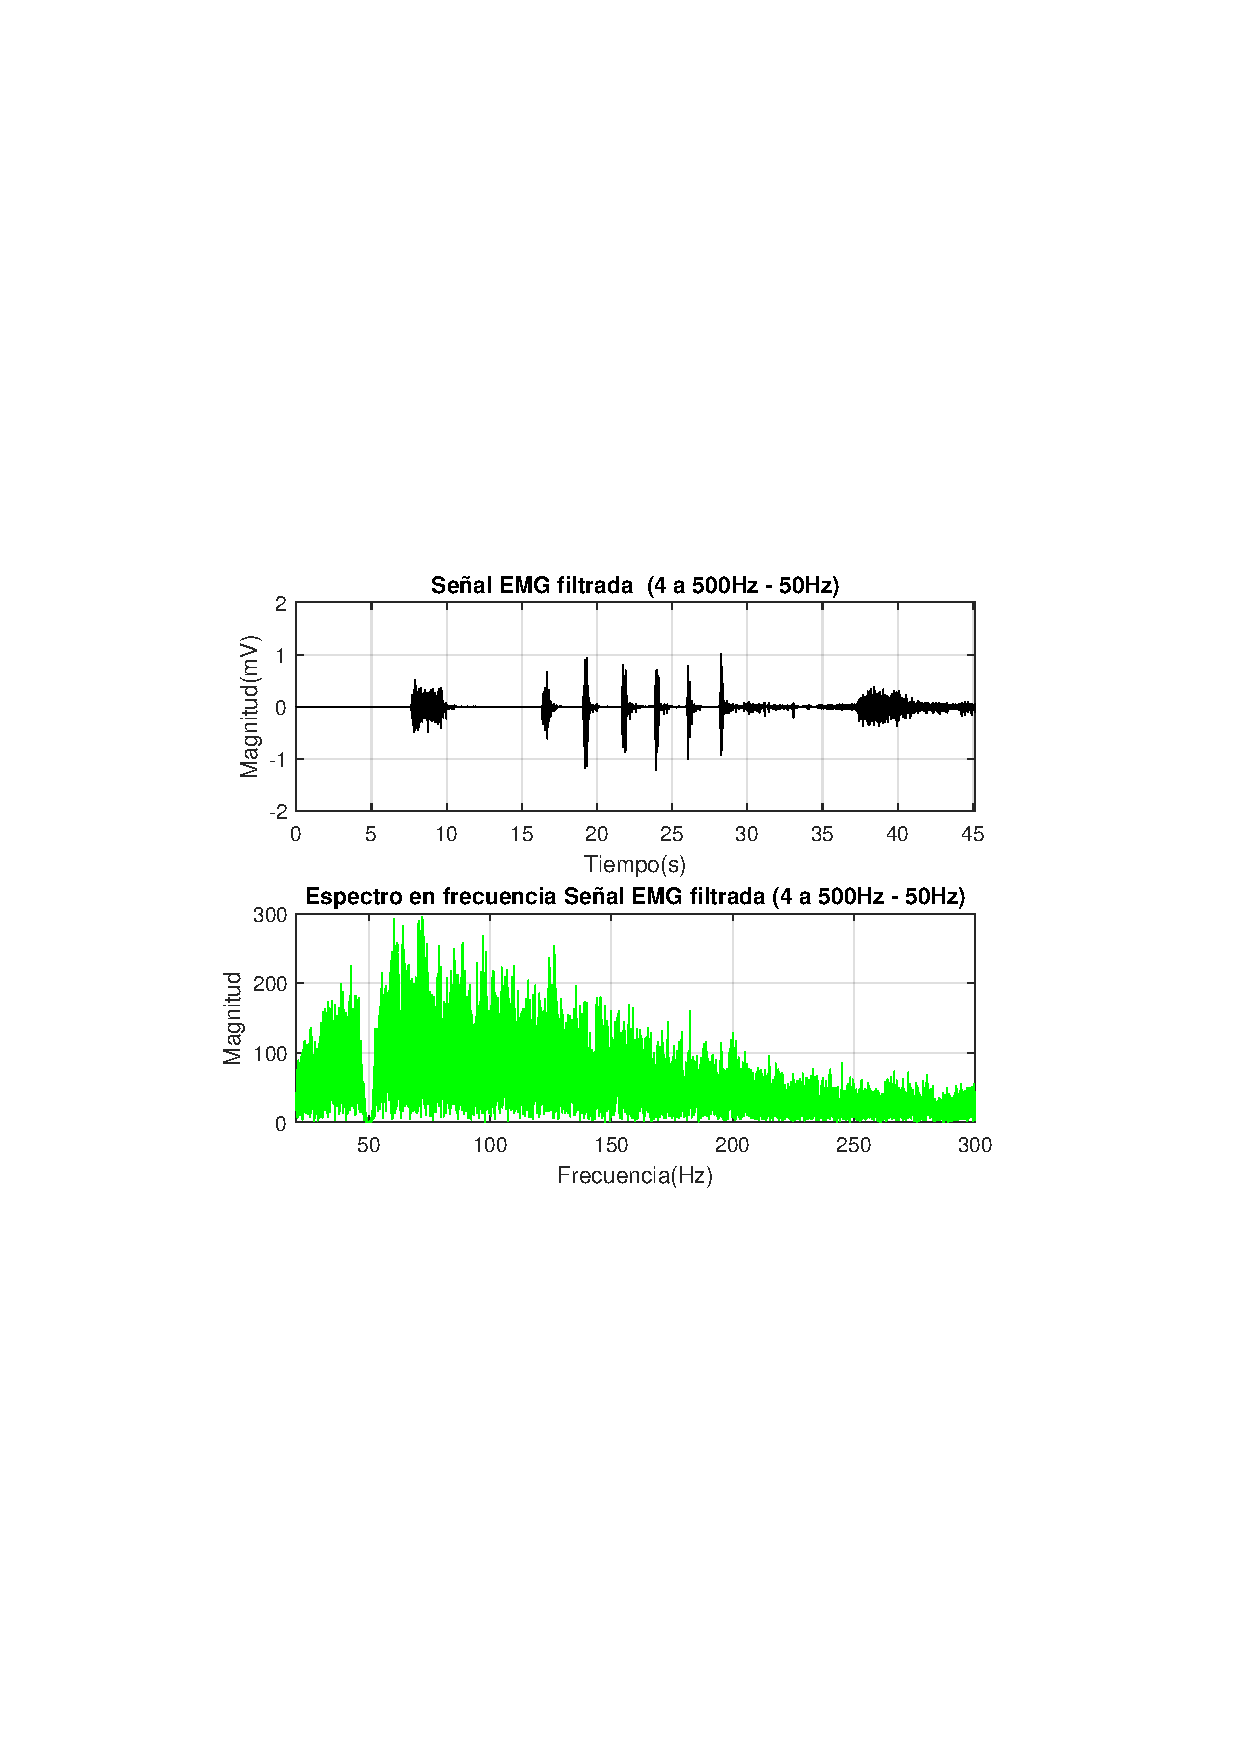
\includegraphics[scale=0.5]{imagenes/Disenodelsistema/graf3.png}
	\caption{Señal con el filtro paso banda y el rechazo banda}
	\label{fig:graf3}
\end{figure}

Haciendo la comparación de la señal antes y después del filtrado, se puede ver el resultado de los filtros. En la figura \ref{fig:graf4} se representa en rojo la señal original y en negro la señal una vez acondicionada. 

\begin{figure}[H]
	\center
	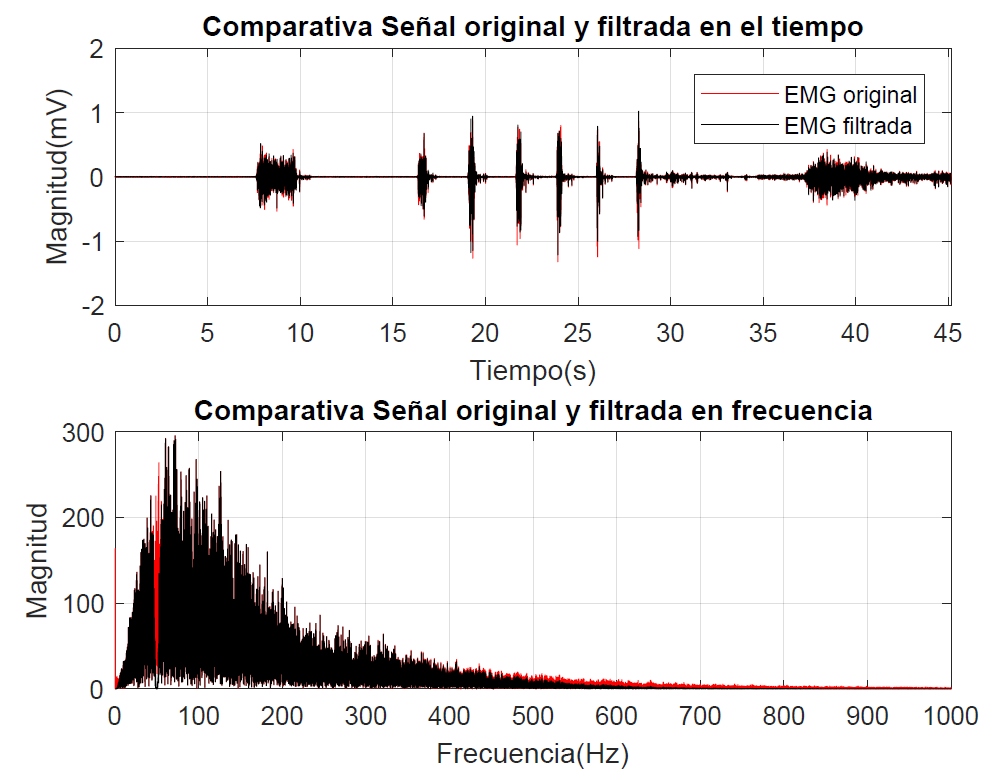
\includegraphics[scale=0.5]{imagenes/Disenodelsistema/graf4.png}
	\caption{Comparativa antes y después del los filtros}
	\label{fig:graf4}
\end{figure}

\subsubsection{Caracterización de la señal}

Una vez la señal está acondicionada adecuadamente, se implementan técnicas de caracterización para sacar parámetros que nos permitan reconocer los distintos movimientos. Se necesitan herramientas para obtener la energía promedio de la señal que nos permitan caracterizar los distintos cambios que sufre esta dependiendo de la contracción.
La señal EMG es muy oscilante (puede cambiar rápidamente en un milisegundo) por lo que resultaría imposible utilizarla directamente para controlar un sistema robótico. Se necesita un método que permita obtener características de la señal y poder definir patrones o comportamientos de ésta. \newline

Una manera de caracterizar una señal es usando el \textit{método por ventanas} que calcula la envolvente de la señal EMG. Para ello dividimos la señal en segmentos o ventanas de longitud L de 250ms con un solapamiento entre ventanas de 125ms, y caracterizamos usando la \textit{Suma de valores absolutos} o \textit{IAV}. Cuanto menor sea L y más alto el solapamiento, mayor número de ventanas y mejor caracterización; pero el procesamiento será más lento. \newline

La IAV \textit{suma de valores absolutos} realiza la suma de los valores absolutos contenidos en cada una de las secciones o ventanas en las que hemos dividido la señal, para dar una idea aproximada de la intensidad de esa ventana. \newline


 La expresión de la IAV se define en \ref{eqn:ec2}:

\begin{equation}
EMG_IAV=\sum_{k=1}^{N}|EMG_{k}|, i=0,......,L-1.
\label{eqn:ec2}
\end{equation}

Esto nos permite distinguir mediante umbrales los grados de intensidad de la señal obtenida, cuanto más tensión se aplique más energía tendrá la señal EMG, lo que se traducirá en un pico más grande de la IAV.
Con esto ya podemos decir que si una señal pasa determinado umbral será una contracción fuerte, contracción leve o relajación.

\begin{figure}[H]
	\center
	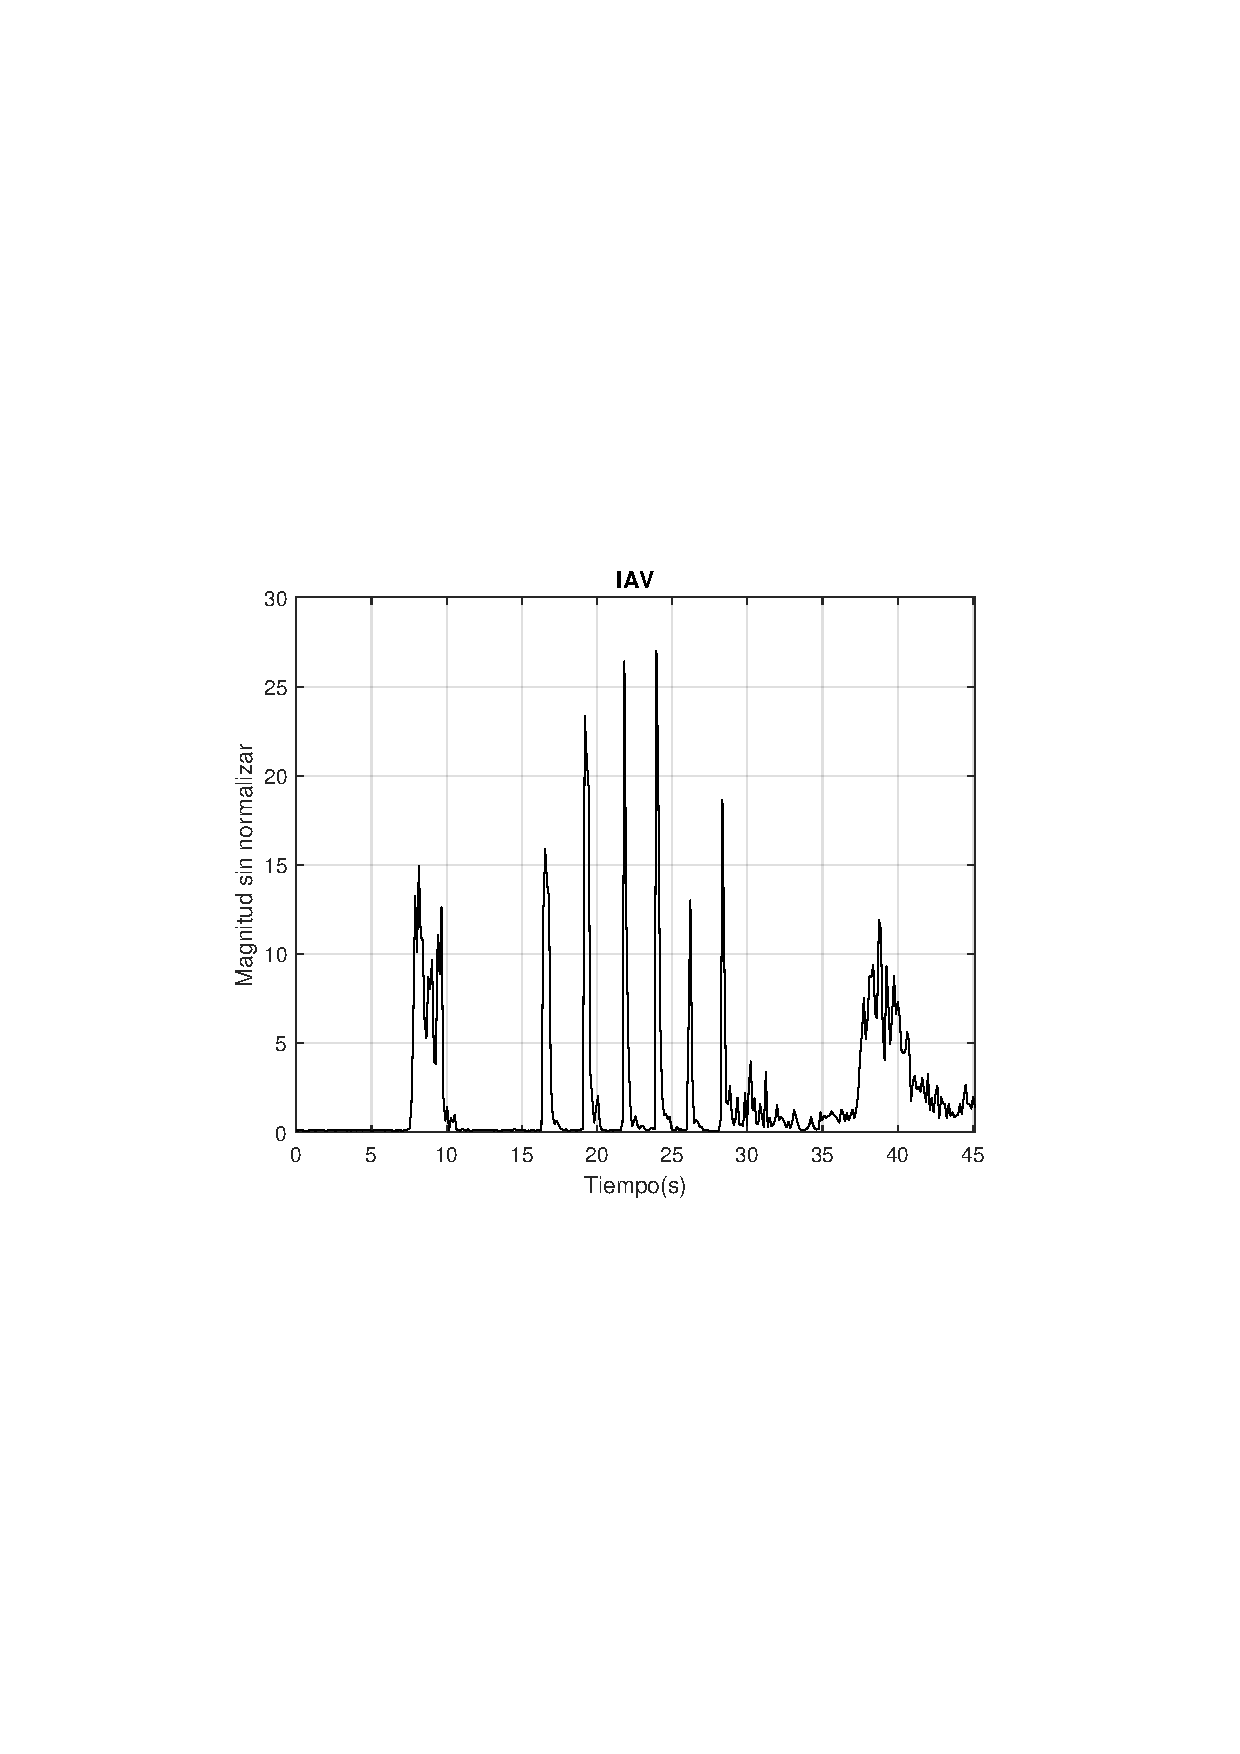
\includegraphics[scale=0.5]{imagenes/Disenodelsistema/graf5.png}
	\caption{Representación de la IAV}
	\label{fig:graf5}
\end{figure}

\subsubsection{Testeo del algoritmo}

Para el testeo del algoritmo se propone usar varias señales tomadas posteriormente,sin modificar el algoritmo de procesamiento. Para ello recogemos una serie de señales de pruebas, en concreto 10 con el brazo derecho y 10 con el brazo izquierdo. Se ha tratado de realizar en todos las señales captadas los mismos movimientos a diferentes velocidades y orden, para ver si el algoritmo es capaz de distinguirlos correctamente.  \newline

En principio nos interesa poder identificar en las señales tres movimientos con cada brazo, que tendrán distintos niveles de tensión para el músculo.

	\begin{itemize}
	\item \textbf{El músculo relajado.} En el que la contracción, y por lo tanto la IAV será mínima.
	\item \textbf{El músculo contraído levemente.} La IAV presentará mayor amplitud.
	\item \textbf{El músculo contraído y con el brazo girado.} La contracción será máxima y mucho mayor la IAV que en los otros dos movimientos.
	\end{itemize}

En la tabla \ref{tabla:tabla1} recogemos las pruebas hechas con el algoritmo para las diferentes señales captadas con cada brazo. El algoritmo es capaz de procesar y discriminar cada señal correctamente. 

\renewcommand\tablename{Tabla}
\begin{table}[H]
\centering
\begin{tabular}{|l|l|l|l|l|}
\hline
\multicolumn{2}{|l|}{}                       & Relajación & Contracción & Giro \\ \hline
\multirow{10}{*}{Brazo derecho}   & Señal 1  & OK         & OK          & OK   \\ \cline{2-5} 
                                  & Señal 2  & OK         & OK          & OK   \\ \cline{2-5} 
                                  & Señal 3  & OK         & OK          & OK   \\ \cline{2-5} 
                                  & Señal 4  & OK         & OK          & OK   \\ \cline{2-5} 
                                  & Señal 5  & OK         & OK          & OK   \\ \cline{2-5} 
                                  & Señal 6  & OK         & OK          & OK   \\ \cline{2-5} 
                                  & Señal 7  & OK         & OK          & OK   \\ \cline{2-5} 
                                  & Señal 8  & OK         & OK          & OK   \\ \cline{2-5} 
                                  & Señal 9  & OK         & OK          & OK   \\ \cline{2-5} 
                                  & Señal 10 & OK         & OK          & OK   \\ \hline
\multirow{10}{*}{Brazo izquierdo} & Señal 1  & OK         & OK          & OK   \\ \cline{2-5} 
                                  & Señal 2  & OK         & OK          & OK   \\ \cline{2-5} 
                                  & Señal 3  & OK         & OK          & OK   \\ \cline{2-5} 
                                  & Señal 4  & OK         & OK          & OK   \\ \cline{2-5} 
                                  & Señal5   & OK         & OK          & OK   \\ \cline{2-5} 
                                  & Señal 6  & OK         & OK          & OK   \\ \cline{2-5} 
                                  & Señal 7  & OK         & OK          & OK   \\ \cline{2-5} 
                                  & Señal 8  & OK         & OK          & OK   \\ \cline{2-5} 
                                  & Señal 9  & OK         & OK          & OK   \\ \cline{2-5} 
                                  & Señal 10 & OK         & OK          & OK   \\ \hline
\end{tabular}
	\caption{Señales de prueba y resultados}
	\label{tabla:tabla1}
\end{table}
\newpage

\subsection{Comunicación serie en Matlab}

Una vez procesadas las señales tenemos que pasarlas a la FPGA para el diseño del sistema de control. El \textit{puerto serie} nos abre la posibilidad de comunicar el ordenador con nuestros circuitos en la FPGA, y por lo tanto poder enviar datos de x bits. Se trata de comunicaciones serie asíncronas y se utiliza un único cable de datos para recepción y transmisión. Tras la clasificación de las señales con la IAV ajustamos el rango de datos obtenido de 0 a 255  (8bits) en Matlab y estos se envían mediante el puerto serie (COM7) a la FPGA.\newline

Para ello será necesario abrir el puerto serie del ordenador con el comando \textit{fopen}, enviar los datos con \textit{fwrite} y definir la velocidad de transmisión, que será para toda la transmisión y recepción de 115200 baudios.

\section{Diseño en icestudio}

\subsection{Receptor serie}\label{sec:rserie}

La FPGA icezum Alhambra que vamos a utilizar ofrece a través del USB una interfaz de comunicaciones serie síncronas (por la que se realiza la carga del programa creado en Icestudio a la placa) y una interfaz de puerto serie. Por lo tanto para realizar la conexión entre PC-FPGA bastaría con conectarlos mediante un USB para tener listo el hardware de envío de datos. No solo es necesario abrir el puerto serie por Matlab, también la FPGA necesita para recibirlos un receptor serie, que habrá que crearlo en Icestudio.\newline

El esquema del receptor de bits mediante el puerto serie planteado se muestra en la figura \ref{fig:receptorserie}:

\begin{figure}[H]
	\center
	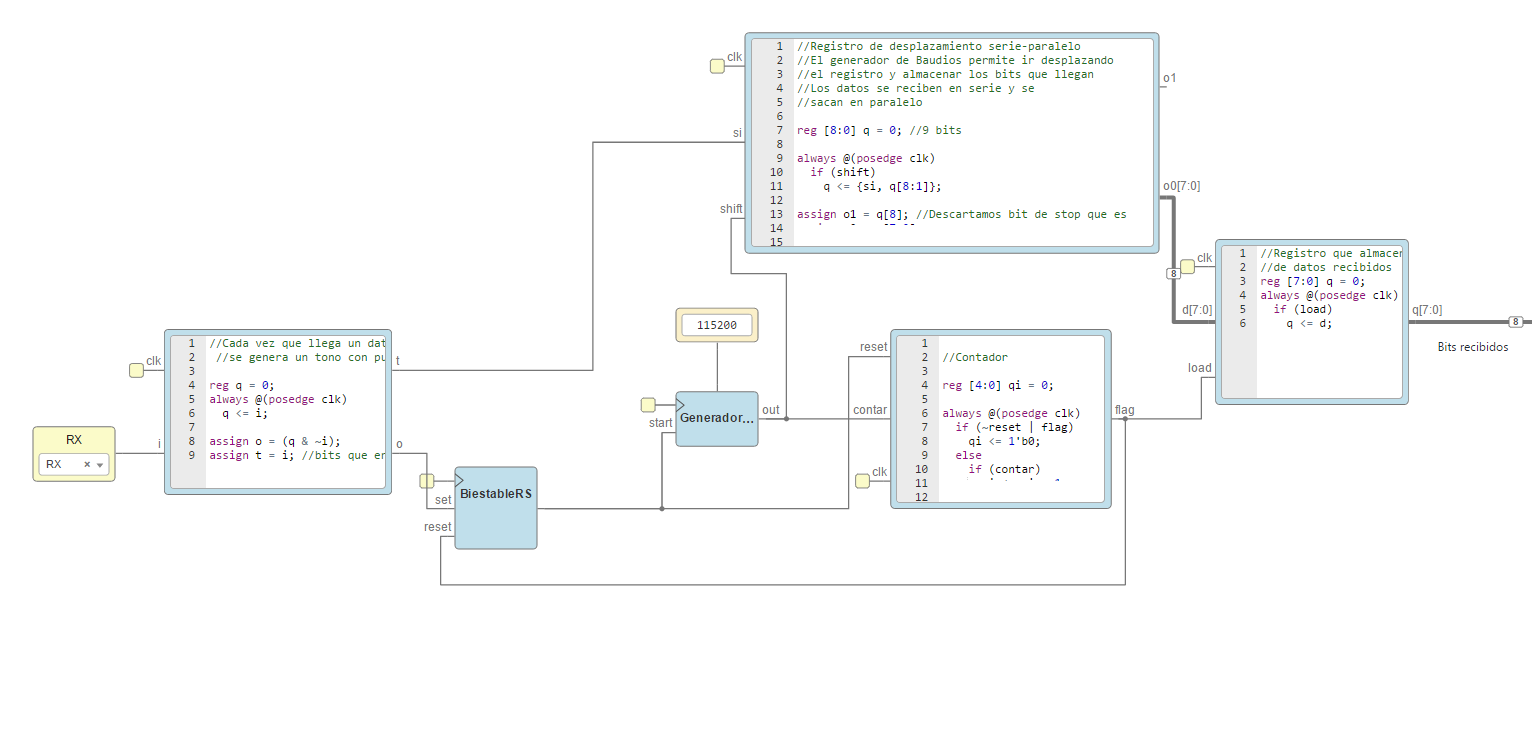
\includegraphics[scale=0.5]{imagenes/Disenodelsistema/receptorserie.png}
	\caption{Receptor serie en icestudio}
	\label{fig:receptorserie}
\end{figure}

Los bits deben de llegar por el puerto serie y salir por un bus de 8 bits  en paralelo para poder utilizar los datos que llegan. 
\begin{figure}[H]
	\center
	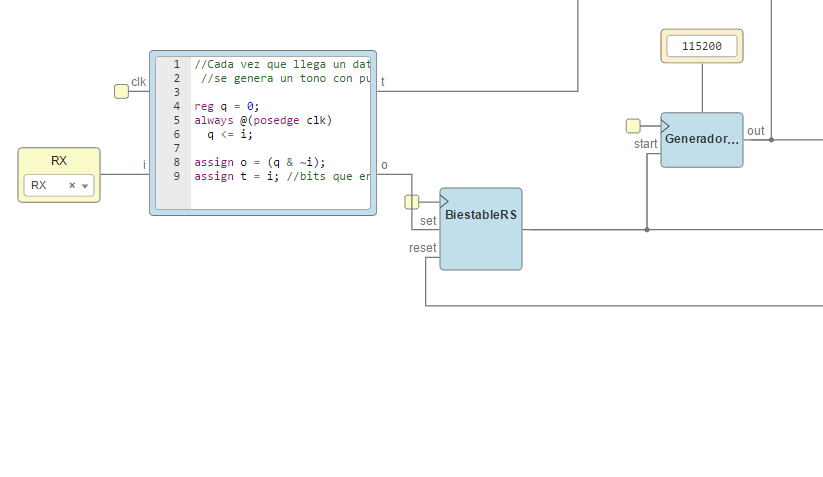
\includegraphics[scale=0.7]{imagenes/Disenodelsistema/receptorserie1.png}
	\caption{Primera parte del receptor serie}
	\label{fig:receptorserie1}
\end{figure}

Por RX llegan los bits en tramas en serie, primero el bit de start, después los bits empezando por el menos significativo y luego el bit de stop. Cada vez que llega un bit de start (que una trama es enviada) se genera un tono puro que activa un biestable RS; el cuál se reseteará para recibir un nuevo dato. Éste a su vez activa un generador de baudios a la velocidad de recepción serie de 115200 baudios.\newline
\begin{figure}[H]
	\center
	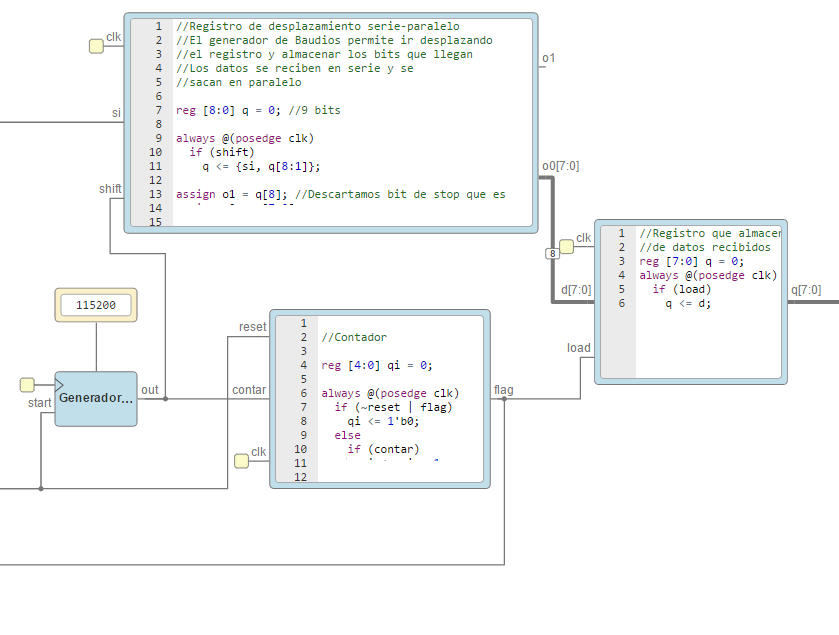
\includegraphics[scale=0.7]{imagenes/Disenodelsistema/receptorserie2.png}
	\caption{Segunda parte del receptor serie}
	\label{fig:receptorserie2}
\end{figure}


Con el generador de baudios se generan los tics para leer los bits serie que van llegando a una velocidad determinada. La salida del generador va a un registro de desplazamiento serie-paralelo y a un contador.El generador de Baudios permite ir desplazando el registro y almacenar los bits que llegan.Los datos se reciben en serie y se sacan en paralelo.A su vez que el generador de baudios genera un tic se incrementa el contador. Al llegar a 9 bits ( 8 datos y 1 stop- el de start solo es para arrancar) significa que ya ha llegado el dato completo y se  activa el flag que reinica el biestable RS y se queda listo para recibir un nuevo dato.
\subsection{Modulador de PWM}

Como hemos visto en \ref{sec:comdron} el dron necesita recibir las señales mediante un protocolo de comunicaciones. Por lo tanto habrá que adaptar las señales recibidas en la FPGA a una modulación PWM. \newline

La Modulación por anchura de pulsos nos va a permitir generar señales analógicas a partir de sistemas digitales.  Esto se puede usar por ejemplo para mover un motor a diferentes velocidades, o cambiar la intensidad con la que brilla un led. Para nuestra aplicación nos va a permitir enviarle las órdenes al dron, y definir un sistema de control en base a las señales que hemos obtenido con el receptor serie. \ref{sec:rserie}

Para ello se ha creado el bloque PWM de la figura \ref{fig:bloquepwm}

\begin{figure}[H]
	\center
	\includegraphics[scale=0.7]{imagenes/Disenodelsistema/bloquePWM.png}
	\caption{Bloque PWM}
	\label{fig:bloquepwm}
\end{figure}

Para cada entrada de datos de 8 bits se genera una señal de PWM en la salida. La estructura del bloquePWM es la siguiente:

\begin{figure}[H]
	\center
	\includegraphics[scale=0.5]{imagenes/Disenodelsistema/bloquePWM2.png}
	\caption{Estructura del Bloque PWM}
	\label{fig:bloquepwm2}
\end{figure}

Ésta cuenta con 2 elementos principales:

	\begin{itemize}
	\item \textbf{Un contador de reloj.} El contador tiene N bits. N va a determinar la frecuencia y tendremos que elegirla por lo tanto antes de el diseño del contador
	\item \textbf{Un registro de anchura.} El valor de anchura de pulso será el dato que llega por la entrada; es la información que se recibe del sistema de adquisición.
	\end{itemize}

La frecuencia que tenga la señal PWM por lo tanto, podremos obtenerla a partir de la señal de reloj del sistema de 12 MHz con un divisor de frecuencia. Para ello tenemos que tener en cuenta la frecuencia que deseemos, que se presentan en la tabla \ref{tabla:tabla2}.

\begin{table}[H]
\centering
\begin{tabular}{lll}
\hline
 \multicolumn{1}{|l|}{Frecuencia} & \multicolumn{1}{l|}{Reloj(S)}                      \\ \hline
 \multicolumn{1}{|l|}{12 MHZ}     & \multicolumn{1}{l|}{S}                             \\ \hline
 \multicolumn{1}{|l|}{6 MHZ}      & \multicolumn{1}{l|}{S/2}                           \\ \hline
 \multicolumn{1}{|l|}{3 MHZ}      & \multicolumn{1}{l|}{S/4}                           \\ \hline
 \multicolumn{1}{|l|}{1.5 MHZ}    & \multicolumn{1}{l|}{S/8}                           \\ \hline
 \multicolumn{1}{|l|}{750 KHZ}    & \multicolumn{1}{l|}{S/16}                          \\ \hline
 \multicolumn{1}{|l|}{375 KHZ}    & \multicolumn{1}{l|}{S/32}                          \\ \hline
 \multicolumn{1}{|l|}{187.5 KHZ}  & \multicolumn{1}{l|}{S/64}                          \\ \hline
 \multicolumn{1}{|l|}{93.8 KHZ}   & \multicolumn{1}{l|}{S/128}                         \\ \hline
 \multicolumn{1}{|l|}{46.9 KHZ}   & \multicolumn{1}{l|}{S/256}                         \\ \hline
 \multicolumn{1}{|l|}{23.4 KHZ}   & \multicolumn{1}{l|}{S/512} \\ \hline
 \multicolumn{1}{|l|}{11.7 KHZ}   & \multicolumn{1}{l|}{S/1024}    \\ \hline
 \multicolumn{1}{|l|}{5.9 KHZ}    & \multicolumn{1}{l|}{S/2048}                        \\ \hline
 \multicolumn{1}{|l|}{2.9 KHZ}    & \multicolumn{1}{l|}{S/4096}                        \\ \hline
 \multicolumn{1}{|l|}{1.5 KHZ}    & \multicolumn{1}{l|}{S/8192}                        \\ \hline
 \multicolumn{1}{|l|}{732 Hz}     & \multicolumn{1}{l|}{S/16384}                       \\ \hline
 \multicolumn{1}{|l|}{366 Hz}     & \multicolumn{1}{l|}{S/32768}                       \\ \hline
 \multicolumn{1}{|l|}{183 Hz}     & \multicolumn{1}{l|}{S/65536}                       \\ \hline
 \multicolumn{1}{|l|}{92 Hz}      & \multicolumn{1}{l|}{S/131072}                      \\ \hline                                                  
\end{tabular}
	\caption{Frecuencias y Reloj del sistema}
	\label{tabla:tabla2}
\end{table}

Si queremos por ejemplo una señal PWM de 92 Hz, tenemos que usar un contador de 17 bits \ref{eqn:reloj}. Esta corresponde a un periodo de 11ms aproximadamente, que será el que usemos para nuesta aplicación.

\begin{equation}
Bits(N)= \frac{Reloj del sistema(12Mhz)} {131072}=17 bits.
\label{eqn:reloj}
\end{equation}

En el divisor de frecuencias los 8 bits más significativos se extraen y estos se comparan con los 8 bits que llegan del registro de anchura W. Esta comparación es lo que permite generar los ciclos de PWM.

	\begin{itemize}
	\item Si el contador es \textbf{menor} que el registro de anchura. La salida será 1.
	\item Si contador es \textbf{mayor} que el registro de anchura . La salida será 0.
	\end{itemize}
%\chapter{Implementación del sistema}\label{sec:Implementacion}

\section{Adquisición}


En la adquisición de señales EMG hay que tener en cuenta un correcto acondicionamiento tanto como de la piel como del sistema.


\subsection{Preparación de la piel} \label{sec:Preparaciondelapiel}
 Es necesario a la hora de obtener señales EMG una correcta preparación de la piel dónde vamos a colocar los electrodos; de forma que la calidad de la señal obtenida sea la mejor posible. Para este propósito es recomendable usar un gel abrasivo o alcohol tanto para eliminar las células muertas de la piel como para reducir la sequedad de la misma. Tras la correcta limpieza con un paño suave se asegura que la zona quede totalmente limpia y seca. \newline
\subsection{Los electrodos} \label{sec:Loselectrodos}

Para ello se usan 3 electrodos  (2 y uno de referencia) que se colocan directamente sobre la piel y son capaces de captar la actividad bioeléctrica. La ubicación de los electrodos va a influir directamente sobre la calidad de las señales obtenidas; una correcta colocación sería en paralelo a las fibras musculares, en la zona central del músculo del que queramos obtener la actividad eléctrica. Estos deberán estar separados de 1 a 2 cm y el de referencia deberá estar colocado en un sitio dónde sepamos que la actividad será minima. En los tendones y el borde del músculo las fibras musculares se vuelven más delgadas y pequeñas por lo que son el sitio ideal para colocar el electrodo de referencia. 

Antes de colocar los electrodos se puede usar una pasta conductiva que mejora considerablemente la captación de estos de las señales.\newline

\begin{figure}[H]
	\center
	\includegraphics[scale=0.8]{imagenes/Implementaciondelsistema/electrodo.png}
	\caption{Posición de los electrodos}
	\label{fig:Posicion}
\end{figure}

\subsection{Captación de señales}

En la captación por lo tanto de señales EMG, con lo visto en \ref{sec:Preparaciondelapiel} y \ref{sec:Loselectrodos} tendríamos que definir el músculo que va a hacer de instrumento de control para el sistema. Se plantea la idea de usar un músculo del antebrazo por la facilidad para la colocación de los electrodos, así como a la hora de descriminar los distintos movimientos que nos van a permitir el control del sistema. Un correcto sitio sería con los 2 electrodos en la parte central y el de referencia en el codo que es un punto neutro.\newline 

El músculo flexor del carpo (figura \ref{fig:flexor}) será  el que eligiremos debido a su posición central, ya que permite contraerlo y relajarlo con facilidad. \newline Por lo tanto este será el músculo sobre el cual vamos a colocar los electrodos para realizar la toma de señales y empezar a discriminar los distintos movimientos.  

\begin{figure}[H]
	\center
	\includegraphics[scale=0.5]{imagenes/Implementaciondelsistema/flexor.png}
	\caption{Músculo flexor del carpo en el antebrazo}
	\label{fig:flexor}
\end{figure}


 las señales EMG de entrenamiento, que mediante Bluethooth son enviadas al ordenador en tiempo real y vistas en el software OpenSignals. Desde que ponemos en marcha el programa hasta que lo paramos las señales EMG captadas con los electrodos se pueden ver en el mismo programa,y elegir el rango de tiempo que queremos guardar. Estas señales guardadas en el ordenador son procesadas en Matlab para flitrar el rango que nos interesa de frecuencias, para eliminar el ruido y mediante umbrales discriminar si el movimiento es de más o menos intensidad. \newline
Una vez las señales son procesadas son enviadas mediante comunicación serie a la FPGA.



\section{Procesamiento en Matlab}
%
%\input{capitulos/06_Implementacion}
%
%\input{capitulos/07_Pruebas}
%
%\input{capitulos/08_Conclusiones}
%
%%\chapter{Conclusiones y Trabajos Futuros}
%
%
\nocite{*}
%\bibliography{bibliografia/bibliografia}\addcontentsline{toc}{chapter}{Bibliografía}
%\bibliographystyle{miunsrturl}
\bibliographystyle{unsrt}
\bibliography{Bio}
%
%\appendix
%\input{apendices/manual_usuario/manual_usuario}
%%\input{apendices/paper/paper}
%\input{glosario/entradas_glosario}
% \addcontentsline{toc}{chapter}{Glosario}
% \printglossary
\chapter*{}
\thispagestyle{empty}

\end{document}
